\documentclass[utf8,german,fpg,lot,lof,lol]{zihpub}

\usepackage{caption}
\usepackage{datetime}
\usepackage{etoolbox}
\usepackage[acronyms,nonumberlist,nopostdot,toc,savewrites,xindy]{glossaries}
\usepackage[section,newfloat]{minted}
\usepackage[super]{nth}
\usepackage{pgfplots}
\usepackage[binary-units]{siunitx}
\usepackage{tcolorbox}

\usepackage{CJKutf8}
\AtBeginDvi{\input{zhwinfonts}}

\makeglossaries

\newacronym{api}{API}{\textit{application programming interface}}
\newacronym{apu}{APU}{\textit{accelerated processing unit}}

\newacronym{cpu}{CPU}{\textit{central processing unit}}

\newacronym{dsp}{DSP}{\textit{digital signal processor}}

\newacronym{fpga}{FPGA}{\textit{field programmable gate array}}

\newacronym{gpgpu}{GPGPU}{\textit{general purpose computation on graphics processing unit}}
\newacronym{gpu}{GPU}{\textit{graphics processing unit}}

\newacronym{hc}{HC}{\textit{Heterogeneous Compute API}}
\newacronym{hcc}{HCC}{\textit{Heterogeneous Compute Compiler}}
\newacronym{hip}{HIP}{\textit{Heterogeneous-Computing Interface for Portability}}
\newacronym{hpc}{HPC}{\textit{high-performance computing}}
\newacronym{hsa}{HSA}{\textit{Heterogeneous System Architecture}}

\newacronym{numa}{NUMA}{\textit{non-uniform memory access}}

\newacronym{openacc}{OpenACC}{\textit{Open Accelerators}}
\newacronym{opencl}{OpenCL}{\textit{Open Compute Language}}
\newacronym{openmp}{OpenMP}{\textit{Open Multi-Processing}}

\newacronym{rock}{ROCk}{\textit{Radeon Open Compute Kernel driver}}
\newacronym{rocm}{ROCm}{\textit{Radeon Open Compute Platform}}
\newacronym{rocr}{ROCr}{\textit{Radeon Open Compute Platform Runtime}}
\newacronym{roct}{ROCt}{\textit{Radeon Open Compute Thunk Interface}}

\newglossaryentry{kernel}{name = Kernel,
                          description = {Programm, das auf einem Beschleuniger,
                                         wie etwa einer GPU, ausgeführt wird.},
                          plural = Kernel}
\newglossaryentry{host}{name = Host,
                        description = {Gerät, das einen Kernel auf dem Device
                                       ausführen lässt. Üblicherweise das Gerät,
                                       auf dem das Betriebssystem läuft, etwa
                                       ein PC oder ein Knoten auf einem
                                       Superrechner.},
                        plural = Hosts}
\newglossaryentry{device}{name = Device,
                          description = {Gerät, das einen Kernel ausführt. Im
                                         Kontext dieser Arbeit stets eine GPU.},
                          plural = Devices}
\newglossaryentry{singlesource}{name = {single-source compilation},
                                description = {Die Quelltexte für Host und
                                               Device werden gleichzeitig vom
                                               Compiler für die
                                               Zielarchitekturen übersetzt.}}
\newglossaryentry{splitsource}{name = {split-source compilation},
                               description = {Die Quelltexte für Host und
                                              Device werden getrennt kompiliert.
                                              Der Host-Quelltext wird von einem
                                              normalen Compiler übersetzt, der
                                              Device-Quelltext erst zur Laufzeit
                                              des Programms von einem weiteren
                                              Compiler.}}


\newenvironment{code}{\captionsetup{type=listing}}{}
\SetupFloatingEnvironment{listing}{name=Quelltext}

\BeforeBeginEnvironment{minted}{\begin{tcolorbox}}
\AfterEndEnvironment{minted}{\end{tcolorbox}}

\newcommand{\lstfont}[1]{\color{#1}\small\ttfamily}

\author{Jan Stephan}
\title{Innovative Spracherweiterungen für Beschleunigerkarten am Beispiel von
       SYCL, HCC, HIP und CUDA: Untersuchung zu Nutzbarkeit und Performance}
\matno{3755136}
\betreuer{\hspace{0.15mm}Dr.-Ing.\ Bernd Trenkler\\
          \qquad \qquad Matthias Werner, M.Sc.}
\date{31.\ Januar 2019}

\bibfiles{bibliography.bib}
\def\UrlBreaks{\do\/\do-}

% Germanisiere LaTeX
\deftranslation[to=German]{Acronyms}{Abkürzungsverzeichnis}
\deftranslation[to=German]{Glossary}{Glossar}
\renewcommand*{\listlistingname}{Quelltextverzeichnis}

\sisetup{locale = DE}

\fancyhf{}
\fancyhead[L]{Jan Stephan -- Innovative Spracherweiterungen}

\begin{document}

\glsaddall

\printglossary
\printglossary[type=\acronymtype]
%\printglossary[type=nomencl,style=nomenclstyle]

\section{Einleitung}
\label{einleitung}

\subsection{Motivation}
\label{einleitung:motivation}

Das Feld der \gls{gpgpu} ist seit 2006 vor allem durch NVIDIAs CUDA-Plattform
und GPUs geprägt und dominiert worden. Die Konkurrenz (vor allem der
GPU-Hersteller AMD) konnte dem lange Zeit wenig entgegensetzen -- heute
(November 2018) sind NVIDIA-GPUs in fünf der zehn leistungsstärksten
Supercomputer vorhanden, darunter die ersten beiden Plätze. Auf der Liste der
500 leistungsstärksten Supercomputer finden sich mit NVIDIA-GPUs bestückte
Rechner insgesamt 126 Mal, GPUs des größten Konkurrenten AMD kein einziges Mal.
Intels als GPU-Alternative vor- und mittlerweile zugunsten einer noch
unbekannten zukünftigen Plattform (vgl.~\cite{intel2017}) eingestellten
Xeon-Phi-Beschleuniger sind auf dieser Liste noch 30 Mal vertreten.
(vgl.~\cite{top500})

Softwareseitig entstand ab 2008 mit der von Apple entwickelten und vom
Khronos-Industriekonsortium standardisierten \gls{opencl} ein offener und
hardware-übergreifender Konkurrent der CUDA-Plattform, der zunächst von einer
Reihe wichtiger Hersteller (einschließlich NVIDIA) unterstützt wurde. Im 
Gegensatz zu CUDA wurde \gls{opencl} von Anfang an auf verschiedene Arten von
Beschleunigern ausgelegt, wie etwa Systeme mit einem \gls{dsp} oder einem
\gls{fpga}. Mit der Zeit zeigte sich jedoch, dass die Unterstützung durch die
Hersteller mit jeder weiteren Revision des Standards abnahm; so ist die 2011
erschienene \gls{opencl}-Version 1.2 bis heute die neueste Version, die von
NVIDIA und AMD\footnote{AMD unterstützte zwischenzeitlich \gls{opencl} 2.0, ist
jedoch infolge des Umbaus des eigenen Treiber- und Compute-Ökosystems auf
\gls{opencl} 1.2 zurückgegangen.} vollständig unterstützt wird. Lediglich Intel
bietet eine Implementierung eines modernen \gls{opencl}-Standards an, beschränkt
sich dabei aber auf seine CPUs und integrierten GPUs. Eine
\gls{opencl}-Implementierung für die neuesten Produktlinien der Xeon-Phi-Reihe,
\textit{Knights Landing} und \textit{Knights Mill}, existiert nicht, während
\gls{opencl} 1.0 (2008) die einzige verfügbare Version für \gls{fpga}s
darstellt.

Sowohl Khronos als auch AMD versuchen seit einigen Jahren, durch neue
Technologien im Umfeld des \gls{hpc} wieder Anschluss an NVIDIA zu finden. Im
März 2014 stellte Khronos den SYCL-Standard vor, der auf \gls{opencl}s Konzepten
und Portabilität aufbaut, jedoch eine auf C++ basierende, deutlich modernere
und angenehmere Programmierweise bieten soll. AMD folgte im April 2016 mit einer
eigenen, quelloffenen Plattform namens \gls{rocm}, die neben einer
Portabilitätsschicht zu CUDA (\gls{hip}) einen auf AMD-GPUs spezialisierten
C++-Dialekt (\gls{hc}) bietet.

Beide Ansätze befinden sich im Gegensatz zu CUDA noch am Anfang ihrer
Entwicklung und erfahren laufend größere Änderungen sowie Feature-Updates. Eine
vergleichende Untersuchung der bereits verfügbaren Fähigkeiten und Konzepte 
sowohl untereinander als auch im Vergleich zu CUDA ist jedoch möglich und in
der wissenschaftlichen Literatur bisher nicht aufzufinden.

\subsection{Forschungsstand}
\label{einleitung:forschung}

Die wissenschaftliche Literatur betrachtet SYCL vornehmlich als
Abstraktionsschicht über \gls{opencl}. Aus diesem Grund sind Untersuchungen, die
sich direkt auf SYCL fokussieren, relativ selten.

Das im März 2014 veröffentlichte SYCL wurde erstmals im August des selben Jahres
von Trigkas untersucht. Zu diesem Zweck wurde SYCL mit \gls{opencl} und
\gls{openmp} verglichen und auf Intels Xeon-Phi-Beschleunigern ausgeführt.
(vgl.~\cite{trigkas2014})

Cardoso da Silva et al.\ führten im Oktober 2016 ebenfalls einen Vergleich
zwischen SYCL, OpenCL und OpenMP durch, als Hardware kamen hier Intels Xeon-CPUs
zum Einsatz.
(vgl.~\cite{dasilva2016})

Jesenšek stellte 2017 eine SYCL-Implementierung für Intels
Xeon-Phi-Prozessoren und das Betriebssystem Linux vor.
(vgl.~\cite{jesensek2017})

Im Mai 2017 zeigten Goli et al.\, dass SYCL zur Beschleunigung des
Deep-Learning-Frameworks \textit{TensorFlow} eingesetzt werden kann.
(vgl.~\cite{goli2017})

Zur selben Zeit verwendeten Copik und Kaiser SYCL als Backend für das
\gls{hpc}-Programmiermodell \textit{HPX.Compute}.
(vgl.~\cite{copik2017})

Im selben Monat untersuchten Doumoulakis et al.\ die Interoperabilität zwischen
SYCL und \gls{opencl} auf GPUs und \gls{fpga}s.
(vgl.~\cite{doumoulakis2017})

Ebenfalls im selben Monat implementierten Aliaga et al.\ BLAS-Algorithmen auf
der Basis von Ausdrucksbäumen und SYCL.
(vgl.~\cite{aliaga2017})

St Clere Smithe und Potter stellten im Mai 2018 ein energieeffizientes
neuronales Netzwerk vor, das mittels SYCL implementiert wurde.
(vgl.~\cite{stcleresmithe2018})

Gleichzeitig zeigte Fare einen ersten Ansatz, der das Profiling von in SYCL
geschriebenen Anwendungen ermöglicht.
(vgl.~\cite{fare2018})

Zur selben Zeit präsentierten Keryell und Yu eine Untersuchung von
auf SYCL aufbauenden Programmen, die auf \gls{fpga}s ausgeführt werden.
(vgl.~\cite{keryell2018})

Afzal et al.\ lösten im Juli 2018 Maxwell-Gleichungen mit SYCL und verglichen
die Performance mit einer vorherigen Implementierung in der Programmiersprache
C.
(vgl.~\cite{afzal2018})

In der wissenschaftlichen Literatur tauchen die Begriffe \gls{rocm}, \gls{hc}
und \gls{hip} erstmals 2016 auf. Während sich die Arbeiten der ersten
Jahreshälfte vornehmlich mit der \gls{hsa} befassen und \gls{rocm} lediglich als
verwendeten Software-Unterbau erwähnen (vgl.\ etwa \cite{li2016},
\cite{larsson2016}), unternahm Sun im Juli 2016 den vermutlich ersten Vergleich
zwischen \gls{hip} und CUDA (vgl.~\cite{sun2016}. Es folgten viele verschiedene
Leistungsanalysen auf der Basis von \gls{rocm}:

Im September 2016 veröffentlichten Sun et al.\ ihre Benchmark-Suite
\textit{Hetero-Mark}, die vornehmlich die Leistungsfähigkeit von \gls{apu}s
misst und dabei auf \gls{rocm} und \gls{hc} aufsetzt (vgl.~\cite{sunyifan2016}).
Sun et al.\ nutzten \textit{Hetero-Mark} sowie das Framework \textit{DNNMark} im
April 2018 erneut, um \gls{rocm} einer eingehenden Performance-Analyse zu
unterziehen (vgl.~\cite{sun2018}). In die gleiche Richtung geht die im April
2017 von Gómez-Luna et al.\ vorgestellte Benchmark-Suite \textit{Chai}
(vgl.~\cite{gomezluna2017}). 

Im Mai 2017 stellten Hou et al.\ Benchmarks vor, die auf der Ebene der Register,
des L1-Caches und des \textit{shared memory} arbeiteten und in \gls{hc} und
CUDA implementiert wurden. (vgl.~\cite{hou2017})

Im Juli 2017 portierte Konstantinidis seine Sammlung von Micro-Benchmarks, die
die Leistungsfähigkeit von CUDA-\gls{gpu}s auf der Instruktionsebene prüfen,
mit der Hilfe von \gls{hip} auf die \gls{rocm}-Plattform.
(vgl.~\cite{konstantinidis2017})

Im Januar 2018 untersuchten Nobre et al.\ die Performanz und Genauigkeit von
Fließkommazahlen mit halber Präzision auf AMD \gls{gpu}s.
(vgl.~\cite{nobre2018})

\subsection{Zielstellung}
\label{einleitung:zielstellung}

Das Ziel dieser Arbeit ist ein vergleichende Analyse der Programmiermodelle
CUDA, SYCL und \gls{rocm} (bzw.\ \gls{hc} und \gls{hip}) auf GPUs der Hersteller
NVIDIA und AMD. Dabei sollen einerseits die den jeweiligen Modellen zugrunde
liegenden Fähigkeiten und Konzepte verglichen, andererseits die konkret
erreichbare Performanz anhand geeigneter Benchmarks ermittelt werden. Von den so
gewonnenen Erkenntnissen werden Empfehlungen für den zukünftigen Einsatz dieser
Modelle im \gls{hpc}-Umfeld abgeleitet.

\subsubsection{Anmerkung}

Die vollständigen Quelltexte und Ergebnisse der Benchmarks sowie die
\LaTeX-Quelltexte dieser Arbeit sind öffentlich unter dem folgenden Link
erreichbar: \url{https://github.com/j-stephan/fpg}

\section{Übersicht der Spracherweiterungen}

\subsection{CUDA}

\subsubsection{Geschichtliche Entwicklung}

\subsubsection{Programmiermodell}

\subsubsection{Hardware-Unterstützung}

\subsubsection{Ökosystem}

\subsection{ROCm}

\subsubsection{Geschichtliche Entwicklung}

\subsubsection{HCC}

\subsubsection{HIP}

\subsubsection{Hardware-Unterstützung}

\subsubsection{Ökosystem}

\subsection{SYCL}

\subsubsection{Geschichtliche Entwicklung}

\subsubsection{Programmiermodell}

\subsubsection{Implementierungen}

\subsubsection{Ökosystem}

%\section{Konzepte und Methoden}
\label{methoden}

\subsection{Theoretische Konzepte}
\label{methoden:konzepte}

Um von den Spracherweiterungen und ihren unterschiedlichen Konzepten in Bezug
auf die Ausführung von Kerneln und die Speicherhierarchie abstrahieren zu
können, wird in diesem Abschnitt ein theoretisches GPU-Modell vorgestellt.
Dieses umfasst alle für das Verständnis der Benchmarks notwendigen Eigenschaften
einer GPU und lässt sich einfach auf die konkreten Konzepte der
Spracherweiterungen abbilden.

\subsubsection{Arbeitsgruppen und -einheiten}

Bei der Ausführung von Kerneln sind zwei Ebenen zu unterscheiden:

\begin{itemize}
    \item Eine \textbf{Arbeitseinheit} ist eine logische Instanz, die auf einen
          Hardware-Thread eines Multiprozessors abgebildet werden kann.
    \item \textbf{Arbeitsgruppen} umfassen eine unbestimmte Zahl von
          Arbeitseinheiten und werden auf die Multiprozessoren der GPU verteilt.
          Arbeitseinheiten innerhalb einer Gruppe sind untereinander
          möglicherweise asynchron, können aber durch Barrieren synchronisiert
          werden. Durch die Verteilung der Arbeitsgruppen auf die
          Multiprozessoren sind auch die Arbeitsgruppen untereinander asynchron
          und können nicht synchronisiert werden.
\end{itemize}

Die Tabelle~\ref{methoden:konzepte:arbeit:tabelle} zeigt die Abbildung der
hier vorgestellten Konzepte auf die äquivalenten Konzepte der verschiedenen
Plattformen.

\begin{table}[htb]
    \centering
    \begin{tabular}{|c|c|c|c|}
        \hline
        Modell & CUDA / HIP & HC & SYCL\\ \hline
        Arbeitsgruppe & block & tile & work group\\ \hline
        Arbeitseinheit & thread & thread & work item\\ \hline
    \end{tabular}
    \caption{Abbildung der Ausführungskonzepte des Modells auf die
             Entsprechungen der Spracherweiterungen}
    \label{methoden:konzepte:arbeit:tabelle}
\end{table}

\subsubsection{Speicherhierarchie}
\label{methoden:konzepte:speicher}

Das theoretische GPU-Modell kennt drei Ebenen der Speicherhierarchie:

\begin{itemize}
    \item Die höchste Ebene ist der \textbf{globale Speicher}. Er entspricht dem
          globalen (GDDR- oder HBM-) Speicher auf realen GPUs, ist im Modell
          jedoch unendlich groß, während die Zugriffszeit sehr langsam ist.
    \item Die nächste Ebene ist der \textbf{lokale Speicher}. Dieser hat in der
          realen Welt unterschiedlich benannte Entsprechungen
          (siehe Tabelle~\ref{methoden:konzepte:speicher:tabelle}), meint aber
          immer den schnellen Speicher, der einer Arbeitsgruppe zugeordnet ist.
          Er ist in der Kapazität beschränkt und deutlich kleiner als der
          globale Speicher, während er wesentlich schnellere Zugriffe
          ermöglicht.
    \item Auf der untersten Ebene befinden sich die \textbf{Register}, die jeder
          Ausführungseinheit in unbegrenzter Zahl zugeordnet sind. Wie in der
          realen Welt sind sie nicht direkt vom Programmierer ansprechbar. Der
          Modell-Compiler platziert in ihnen lokale Variablen der
          Arbeitseinheiten.
\end{itemize}

\begin{table}[htb]
    \centering
    \begin{tabular}{|c|c|c|c|}
        \hline
        Modell & CUDA / HIP & HC & SYCL\\ \hline
        globaler Speicher & global memory & global memory & global memory\\
        \hline
        lokaler Speicher & shared memory & \texttt{tile\_static} memory &
        local memory \\
        \hline
        Register & register & register & -
    \end{tabular}
    \caption{Abbildung des Speicherkonzepte des Modells auf die Entsprechungen
             der Spracherweiterungen}
    \label{methoden:konzepte:speicher:tabelle}
\end{table}

\subsubsection{Kernelsprache}

Die in den vorherigen Abschnitten entwickelten Konzepte werden für die
theoretische Beschreibung der verwendeten Benchmarks in eine fiktive
Kernel-Sprache integriert. Bei dieser Sprache handelt es sich um normales C++
mit folgenden Erweiterungen:

\begin{itemize}
    \item Das Schlüsselwort \texttt{local} markiert Variablen und Arrays, die im
          lokalen Speicher liegen.
    \item Der Befehl \texttt{synchronize()} wirkt als Barriere innerhalb einer
          Arbeitsgruppe. Es wird garantiert, dass alle vorherigen Zugriffe auf
          den (globalen und lokalen) Speicher und Rechenoperationen
          abgeschlossen wurden, bevor die Arbeitseinheiten die Befehle nach der
          Barriere ausführen können.
    \item Das Schlüsselwort \texttt{num\_groups} ist eine Variable, die die
          Anzahl aller Arbeitsgruppen enthält.
    \item Das Schlüsselwort \texttt{group\_idx} dient der eindeutigen
          Identifikation einer Arbeitsgruppe in Form einer ganzen Zahl. Die
          Indices sind fortlaufend, d.h.\ die erste Arbeitsgruppe hat den
          Index 0, die zweite den Index 1 und die $n$-te Arbeitsgruppe den
          Index $n - 1$.
    \item Das Schlüsselwort \texttt{group\_dim} ist eine Variable, die die
          Anzahl der Arbeitseinheiten einer Gruppe beinhaltet.
    \item Das Schlüsselwort \texttt{unit\_idx} dient der eindeutigen
          Identifikation einer Arbeitseinheit innerhalb einer Arbeitsgruppe. Die
          erste Einheit einer Gruppe trägt den Index 0, die zweite den Index 1
          und die $n$-te Einheit den Index $n - 1$.
    \item Die globale Position einer Arbeitseinheit, also die eindeutige
          Identifikation über Gruppengrenzen hinweg, lässt sich mit Hilfe der
          vorgegebenen Schlüsselworte berechnen:\\
          \texttt{global\_id = group\_idx * group\_dim + unit\_idx}
    \item Vektoren werden in der Form \texttt{typZAHL} notiert, z.B.\
          \texttt{int2} oder \texttt{float4}. Der Zugriff auf die Komponenten
          erfolgt über den Punktoperator und die Angabe des Felds.
          Beispielsweise sind die Komponenten des Vektors \texttt{a} vom Typ
          \texttt{float3} durch \texttt{a.x}, \texttt{a.y} und \texttt{a.z}
          ansprechbar.
\end{itemize}

Alle Indices sind im vorgestellten Modell eindimensional, was für die hier
vorgestellten Benchmarks ausreicht.

\subsection{zcopy-Benchmark}
\label{methoden:zcopy}

Der zcopy-Benchmark geht auf einen Beitrag des Nutzers \textit{njuffa}\footnote{
Vermutlich der NVIDIA-Angestellte Norbert Juffa.} im NVIDIA-Forum zurück. Er
hat das Ziel, die tatsächlich erreichbare Speicherbandbreite des globalen
GPU-Speichers zu ermitteln, indem ein Kernel ausschließlich kombinierte Lese-
und Schreibzugriffe (16 Byte pro Thread) durchführt. (vgl.~\cite{njuffa2017})

Der Benchmark wurde für diese Arbeit übernommen und angepasst:

\begin{itemize}
    \item Es wird sowohl die kombinierte Lese- und Schreibgeschwindigkeit als
          auch die reine Schreibgeschwindigkeit gemessen, da die Kombination
          unter Umständen zusätzlichen Overhead im Speicher-Controller der GPU
          erzeugen kann.
    \item Während der originale Benchmark nur auf 16 Byte pro Thread zugreift,
          wurden im Rahmen dieser Arbeit auch die Bandbreiten für die
          Speichergrößen 4 Byte, 8 Byte und 32 Byte ermittelt.
\end{itemize}

Quelltext~\ref{methoden:zcopy:source} zeigt den Pseudo-Code des eingesetzten
Kernels am Beispiel von 16 Byte pro Thread.

\begin{code}
    \begin{minted}[breaklines,breakafter=\,,escapeinside=||,fontsize=\small]{c++}
void read_write(double2* a, double2* b, size_t num_elems)
{
    int stride = |\textbf{\textcolor{keyword-green}{num\_groups}}| * |\textbf{\textcolor{keyword-green}{group\_dim}}|;
    int global_id = |\textbf{\textcolor{keyword-green}{group\_dim}}| * |\textbf{\textcolor{keyword-green}{group\_idx}}| + |\textbf{\textcolor{keyword-green}{unit\_idx}}|;

    for(int i = global_id; i < num_elems; i += stride)
        b[i] = a[i];
}

void write(double2* b, size_t num_elems)
{
    int stride = |\textbf{\textcolor{keyword-green}{num\_groups}}| * |\textbf{\textcolor{keyword-green}{group\_dim}}|;
    int global_id = |\textbf{\textcolor{keyword-green}{group\_dim}}| * |\textbf{\textcolor{keyword-green}{group\_idx}}| + |\textbf{\textcolor{keyword-green}{unit\_idx}}|;

    for(int i = global_id; i < num_elems; i += stride)
        b[i] = double2{0.0, 0.0};
}
    \end{minted}
    \caption{zcopy-Benchmark}
    \label{methoden:zcopy:source}
\end{code}

\subsection{Reduction-Benchmark}
\label{methoden:reduction}

\subsubsection{Theoretischer Hintergrund}

Die Reduktion eines Arrays ist eines der klassischen Konzepte der parallelen
Programmierung. Mathematisch verbirgt sich dahinter das Reduzieren einer Menge
von Zahlen auf eine kleinere Menge von Zahlen durch eine Funktion. Als Beispiel
sei eine Menge von Zahlen $A = \{a_1, a_2, \dots, a_n\}$ gegeben. Durch die
Summenfunktion lässt sich das Ergebnis $b = \sum\limits_{i = 1}^n a_i$
ermitteln -- in Mengen ausgedrückt wurde $A$ auf $B = \{b\}$ reduziert. Auf
die gleiche Weise ließe sich die Menge $C = \{c\}$ durch eine
Multiplikationsreduktion $c = \prod\limits_{i = 1}^n a_i$ berechnen.

Ein serieller Reduktionsalgorithmus ließe sich in Form einer Schleife schreiben,
die über die Menge der Zahlen iteriert und das Ergebnis der Funktion $\oplus$
für alle aufeinander folgenden Zahlen berechnet:

\begin{algorithmic}[1]
\State $result \gets 0$
\For {$i \gets 1, n$}
    \State $result \gets result \oplus a_i$
\EndFor
\end{algorithmic}

Da die Reihenfolge der Anwendung der Funktion $\oplus$ in diesem Beispiel nicht
relevant ist, lässt sich der Algorithmus einfach parallelisieren, indem eine
Menge von $p$ Arbeitseinheiten $\oplus$ zunächst auf $p$ Paare $(a_i, a_j)$
anwendet, wobei $a_i$ und $a_j$ jeweils genau einmal zugeordnet werden ($a_i$
wird also niemals zweimal verwendet). Im nächsten Schritt führen
$\frac{p}{2}$ Einheiten die Funktion erneut auf den Ergebnissen des vorherigen
Schritts aus, usw. Die Abbildung~\ref{methoden:reduction:viz} visualisiert
den Vorgang für acht Elemente $a_1, \dots, a_8$ auf das Ergebnis $b$ durch vier
Ausführungseinheiten $E_1, \dots, E_4$.

\begin{figure}[htb]
    \centering
    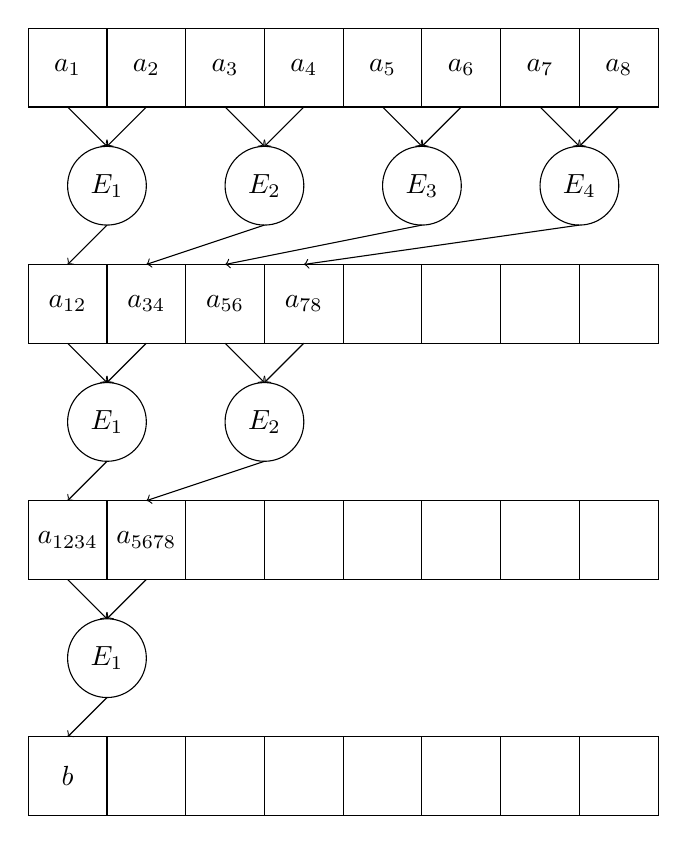
\begin{tikzpicture}
        \draw (0.0, 0.0) rectangle (1.0, -1.0) node [pos = 0.5] {$a_1$};
        \draw (1.0, 0.0) rectangle (2.0, -1.0) node [pos = 0.5] {$a_2$};
        \draw (2.0, 0.0) rectangle (3.0, -1.0) node [pos = 0.5] {$a_3$};
        \draw (3.0, 0.0) rectangle (4.0, -1.0) node [pos = 0.5] {$a_4$};
        \draw (4.0, 0.0) rectangle (5.0, -1.0) node [pos = 0.5] {$a_5$};
        \draw (5.0, 0.0) rectangle (6.0, -1.0) node [pos = 0.5] {$a_6$};
        \draw (6.0, 0.0) rectangle (7.0, -1.0) node [pos = 0.5] {$a_7$};
        \draw (7.0, 0.0) rectangle (8.0, -1.0) node [pos = 0.5] {$a_8$};

        \draw (1.0, -2.0) circle [radius = 0.50] node {$E_1$};
        \draw (3.0, -2.0) circle [radius = 0.50] node {$E_2$};
        \draw (5.0, -2.0) circle [radius = 0.50] node {$E_3$};
        \draw (7.0, -2.0) circle [radius = 0.50] node {$E_4$};

        \draw [->] (0.5, -1.0) -- (1.0, -1.5);
        \draw [->] (1.5, -1.0) -- (1.0, -1.5);
        \draw [->] (2.5, -1.0) -- (3.0, -1.5);
        \draw [->] (3.5, -1.0) -- (3.0, -1.5);
        \draw [->] (4.5, -1.0) -- (5.0, -1.5);
        \draw [->] (5.5, -1.0) -- (5.0, -1.5);
        \draw [->] (6.5, -1.0) -- (7.0, -1.5);
        \draw [->] (7.5, -1.0) -- (7.0, -1.5);

        \draw [->] (1.0, -2.5) -- (0.5, -3.0);
        \draw [->] (3.0, -2.5) -- (1.5, -3.0);
        \draw [->] (5.0, -2.5) -- (2.5, -3.0);
        \draw [->] (7.0, -2.5) -- (3.5, -3.0);

        \draw (0.0, -3.0) rectangle (1.0, -4.0) node [pos = 0.5] {$a_{12}$};
        \draw (1.0, -3.0) rectangle (2.0, -4.0) node [pos = 0.5] {$a_{34}$};
        \draw (2.0, -3.0) rectangle (3.0, -4.0) node [pos = 0.5] {$a_{56}$};
        \draw (3.0, -3.0) rectangle (4.0, -4.0) node [pos = 0.5] {$a_{78}$};
        \draw (4.0, -3.0) rectangle (5.0, -4.0);
        \draw (5.0, -3.0) rectangle (6.0, -4.0);
        \draw (6.0, -3.0) rectangle (7.0, -4.0);
        \draw (7.0, -3.0) rectangle (8.0, -4.0);

        \draw (1.0, -5.0) circle [radius = 0.50] node {$E_1$};
        \draw (3.0, -5.0) circle [radius = 0.50] node {$E_2$};

        \draw [->] (0.5, -4.0) -- (1.0, -4.5);
        \draw [->] (1.5, -4.0) -- (1.0, -4.5);
        \draw [->] (2.5, -4.0) -- (3.0, -4.5);
        \draw [->] (3.5, -4.0) -- (3.0, -4.5);

        \draw [->] (1.0, -5.5) -- (0.5, -6.0);
        \draw [->] (3.0, -5.5) -- (1.5, -6.0);

        \draw (0.0, -6.0) rectangle (1.0, -7.0) node [pos = 0.5] {$a_{1234}$};
        \draw (1.0, -6.0) rectangle (2.0, -7.0) node [pos = 0.5] {$a_{5678}$};
        \draw (2.0, -6.0) rectangle (3.0, -7.0);
        \draw (3.0, -6.0) rectangle (4.0, -7.0);
        \draw (4.0, -6.0) rectangle (5.0, -7.0);
        \draw (5.0, -6.0) rectangle (6.0, -7.0);
        \draw (6.0, -6.0) rectangle (7.0, -7.0);
        \draw (7.0, -6.0) rectangle (8.0, -7.0);

        \draw (1.0, -8.0) circle [radius = 0.50] node {$E_1$};

        \draw [->] (0.5, -7.0) -- (1.0, -7.5);
        \draw [->] (1.5, -7.0) -- (1.0, -7.5);

        \draw [->] (1.0, -8.5) -- (0.5, -9.0);

        \draw (0.0, -9.0) rectangle (1.0, -10.0) node [pos = 0.5] {$b$};
        \draw (1.0, -9.0) rectangle (2.0, -10.0);
        \draw (2.0, -9.0) rectangle (3.0, -10.0);
        \draw (3.0, -9.0) rectangle (4.0, -10.0);
        \draw (4.0, -9.0) rectangle (5.0, -10.0);
        \draw (5.0, -9.0) rectangle (6.0, -10.0);
        \draw (6.0, -9.0) rectangle (7.0, -10.0);
        \draw (7.0, -9.0) rectangle (8.0, -10.0);
    \end{tikzpicture}
    \caption{Visualisierung einer parallelen Reduktion}
    \label{methoden:reduction:viz}
\end{figure}

\subsubsection{GPU-Implementierung}

Im \gls{gpgpu}-Kontext ist die Reduktion früh untersucht worden. So stellte
Harris 2007 eine optimierte Reduktion für CUDA vor (vgl.~\cite{harris2007}). 
Eine für NVIDIAs Kepler-Architektur optimierte Variante der Reduktion wurde 2014
von Luitjens präsentiert (vgl.~\cite{luitjens2014}). Da sich Luitjens'
Implementierung NVIDIA-spezifischer Hardware-Intrinsiken bedient, die nicht auf
jeder im Rahmen dieser Arbeit untersuchten Plattform verfügbar sind, wird hier
ein anderer Ansatz verwendet.

Der Kernel, der die Reduktion durchführt, besteht aus zwei Stufen. Während der
ersten Stufe iterieren $x$ Arbeitsgruppen mit jeweils $p$ Arbeitseinheiten über
den globalen Speicher mit $n$ Elementen. Die Arbeitseinheiten führen die
Reduktion für jedes Elementepaar aus, wobei jeder Iterationsschritt $x \cdot p$
Elemente vom vorherigen Schritt entfernt auf den Speicher zugreift. Unter der
Annahme, dass $n$ ein Vielfaches von $p$ ist, werden $y = \frac{n}{p}$
Arbeitsgruppen gebraucht. Gilt $x \leq y$ unter der Bedingung, dass $y$ ein
Vielfaches von $x$ ist, führt jede Arbeitseinheit die Reduktionsoperation im
ersten Schritt genau $y$-mal aus. Dieses Zugriffsmuster ist als
\textit{(grid-)stride loop} bekannt und ein häufig genutztes Konzept der
\gls{gpgpu}-Programmierung (vgl.~\cite{harris2013} für eine Einführung und
Erklärung der Vorteile).

Während der zweiten Stufe werden die bisherigen Ergebnisse der einzelnen
Arbeitseinheiten in den lokalen Speicher geladen. Dann führt die Hälfte der
Arbeitseinheiten die Reduktionsoperation auf jeweils einem Elementepaar des
lokalen Speichers aus, dann ein Viertel auf der Arbeitseinheiten auf den neuen
Ergebnissen, usw. Am Ende gibt es pro Arbeitsgruppe genau ein Teilergebnis der
Reduktionsoperation (also $x$ Ergebnisse), das wieder in den globalen Speicher
geschrieben wird.

Durch einen erneuten Aufruf des Kernels mit einer Arbeitsgruppe und
$\frac{x}{2}$ Arbeitseinheiten lässt sich in einem weiteren Schritt das
Gesamtergebnis der Reduktion berechnen. Quelltext~\ref{methoden:reduction:code}
zeigt den Pseudo-Code des Kernels.

\begin{code}
    \begin{minted}[breaklines,breakafter=\,,escapeinside=||,fontsize=\small]{c++}
void block_reduce(const int* data, int* result, size_t num_elems)
{
    |\textbf{\textcolor{keyword-green}{local}}| int shared[p];

    int global_id = |\textbf{\textcolor{keyword-green}{group\_idx}}| * |\textbf{\textcolor{keyword-green}{group\_dim}}| + |\textbf{\textcolor{keyword-green}{unit\_idx}}|;
    int tsum = data[global_id]; // vermeide neutrales Element
    int grid_size = |\textbf{\textcolor{keyword-green}{group\_dim}}| * |\textbf{\textcolor{keyword-green}{num\_blocks}}|;
    global_id += grid_size;

    // 1. Stufe: grid-stride loop
    while((global_id + 3 * grid_size) < num_elems)
    {
        tsum += data[global_id] + data[global_id + grid_size] +
                data[global_id + 2 * grid_size] +
                data[global_id + 3 * grid_size];
        i += 4 * grid_size;
    }

    // verbleibende Elemente, falls n kein Vielfaches von p ist
    while(global_id < num_elems)
    {
        tsum += data[global_id];
        global_id += grid_size;
    }

    // schreibe Ergebnis in lokalen Speicher
    shared[|\textbf{\textcolor{keyword-green}{unit\_idx}}|] = tsum; 
    |\textbf{\textcolor{keyword-green}{synchronize}}|();

    // 2. Stufe: Reduktion innerhalb der Gruppe
    for(int bs = |\textbf{\textcolor{keyword-green}{group\_dim}}|, bsup = (|\textbf{\textcolor{keyword-green}{group\_dim}}| + 1) / 2;
        bs > 1;
        bs /= 2, bsup = (bs + 1) / 2)
    {
        bool cond = |\textbf{\textcolor{keyword-green}{unit\_idx}}| < bsup // erste Gruppenhälfte
            && |\textbf{\textcolor{keyword-green}{unit\_idx}}| + bsup < |\textbf{\textcolor{keyword-green}{group\_dim}}|
            && (|\textbf{\textcolor{keyword-green}{group\_idx}}| * |\textbf{\textcolor{keyword-green}{group\_dim}}| + |\textbf{\textcolor{keyword-green}{unit\_idx}}| + bsup) < num_elems;

        if(cond) shared[|\textbf{\textcolor{keyword-green}{unit\_idx}}|] += shared[|\textbf{\textcolor{keyword-green}{unit\_idx}}| + bsup];
        |\textbf{\textcolor{keyword-green}{synchronize}}|();
    }
    
    // Ergebnis in globalen Speicher schreiben
    if(|\textbf{\textcolor{keyword-green}{unit\_idx}}| == 0) result[|\textbf{\textcolor{keyword-green}{group\_idx}}|] = shared[0];
}
    \end{minted}
    \caption{Reduction-Benchmark}
    \label{methoden:reduction:code}
\end{code}

\subsection{N-Body-Benchmark}
\label{methoden:nbody}

\subsubsection{Vorbemerkung}
\label{methoden:nbody:vorbemerkung}

Eine effiziente Implementierung einer N-Body-Simulation mit quadratischer
Komplexität für GPUs wurde 2007 von Nyland et al.\ vorgestellt. Der in dieser
Arbeit verwendete Benchmark folgt dieser Implementierung, die theoretische
Beschreibung ist (gekürzt) ebenfalls der Arbeit von Nyland et al.\ entnommen.
(vgl.~\cite{nguyen2007})

\subsubsection{Einführung}
\label{methoden:nbody:einfuehrung}

N-Body-Simulationen wenden numerische Methoden an, um die Entwicklung eines
Systems vieler miteinander interagierender Körper zu approximieren.
N-Body-Probleme sind in den Naturwissenschaften zahlreich vertreten,
beispielsweise bei der Simulation vieler Galaxien oder Sterne und deren
Wechselwirkungen durch die Schwerkraft.

Eine N-Body-Simulation aller Körperpaare ist eine \textit{brute-force}-Technik,
die alle paarweisen Interaktionen auswertet. Aufgrund der quadratischen
Komplexität $\mathcal{O}(n^2)$ ist die Rechenlast bei großen Systemen sehr hoch:
ein System mit \num{16384} Körpern, das 20 Zeitschritte pro Sekunde simuliert,
berechnet über fünf Milliarden Interaktionen pro Sekunde. Aus diesem Grund ist
eine solche Simulation ein interessantes Ziel für den Einsatz paralleler
Beschleuniger.

\subsubsection{Mathematischer Hintergrund}
\label{methoden:nbody:mathematik}

In der in dieser Arbeit verwendeten Simulation wird das Gravitationspotential
aller Körper berechnet. Die in den folgenden Formeln vorkommenden Vektoren
werden in der Form $\vec{a}, \vec{b}, \vec{c}$ notiert und sind grundsätzlich
dreidimensional.

In einem System aus $N$ Körpern mit der Startposition $\vec{x}_i$ und der
Geschwindigkeit $\vec{v}_i$ ($1 \leq i \leq N$) ergibt sich die auf den Körper
$i$ durch die Anziehungskraft des Körpers $j$ wirkende Kraft $\vec{f}_{ij}$ wie
folgt:

\[
    \vec{f}_{ij} = G \frac{m_i m_j}{|\vec{r}_{ij}|^2} \cdot
                   \frac{\vec{r}_{ij}}{|\vec{r}_{ij}|},
\]

wobei $m_i$ und $m_j$ die Massen der Körper $i$ und $j$ sind,
$\vec{r}_{ij} = \vec{x}_j - \vec{x}_i$ der Vektor vom Körper $i$ zum Körper $j$
ist und $G$ die Gravitationskonstante darstellt. Der linke Faktor -- der
\textit{Betrag} der Kraft -- ist proportional zum Produkt der Massen und
schrumpft mit zunehmendem Abstand zwischen den Körpern $i$ und $j$. Der rechte
Faktor ist die \textit{Richtung} der Kraft. Aufgrund der anziehenden Wirkung
zwischen den Körpern $i$ und $j$ ist dieser Vektor ist ein Einheitsvektor.

Die gesamte auf den Körper $i$ wirkende Kraft $\vec{F}_i$, die sich aus den
Interaktionen mit den anderen $N - 1$ Körpern ergibt, ist die Summe aller
Interaktionen:

\[
    \vec{F}_i = \sum\limits_{\substack{1 \leq j \leq N\\ j \neq i}} \vec{f}_{ij}
              = G m_i \cdot \sum\limits_{\substack{1 \leq j \leq N\\j \neq i}}
                \frac{m_j \vec{r}_{ij}}{|\vec{r}_{ij}|^3}.
\]

Wenn sich Körper einander nähern, wächst die zwischen ihnen wirkende Kraft bis
ins Unendliche, was bei der numerischen Integration unerwünscht ist. In
astrophysikalischen Simulationen werden daher Kollisionen zwischen Körpern
grundsätzlich ausgeschlossen. Aus diesem Grund wird ein Schwächungsfaktor
$\varepsilon^2 > 0$ hinzugefügt und der Nenner wie folgt umgeschrieben:

\[
    \vec{F}_i \approx G m_i \cdot \sum\limits_{1 \leq j \leq N}
                      \frac{m_j \vec{r}_{ij}}
                           {\sqrt{|\vec{r}_{ij}|^2 + \varepsilon^2}^3}.
\]

Die Bedingung $j \neq i$ wird bei der Summe nicht länger benötigt, da
$\vec{f}_{ii} = 0$, wenn $\varepsilon^2 > 0$. Der Schwächungsfaktor stellt die
Interaktion zwischen zwei Plummer-Massepunkten dar, also Massen, die sich wie
kugelförmige Galaxien verhalten (vgl.~\cite{aarseth2003} und \cite{dyer1993}).
Effektiv beschränkt der Schwächungsfaktor die Größe der Kräfte zwischen Körpern,
was bei der numerischen Integration wünschenswert ist.

Um über die Zeit zu integrieren, muss die Beschleunigung
$\vec{a}_i = \frac{\vec{F}_i}{m_i}$ auf die Position und Geschwindigkeit des
Körpers $i$ angewendet werden, wodurch sich die Berechnung weiter vereinfacht:

\[
    \vec{a}_i \approx G \cdot \sum\limits_{1 \leq j \leq N}
                      \frac{m_j \vec{r}_{ij}}
                           {\sqrt{|\vec{r}_{ij}|^2 + \varepsilon^2}^3}
\]

Der numerische Integrator, der die Positionen und Geschwindigkeiten
aktualisiert und auch in dieser Arbeit zum Einsatz kommt, ist ein
Leapfrog-Verlet-Integrator (vgl.~\cite{verlet1967}). Er ist auf dieses Problem
anwendbar und berechnungseffizient, d.h. die Genauigkeit ist im Verhältnis zum
Rechenaufwand hoch. Die Wahl der Integrationsmethode für N-Body-Simulationen
hängt vom beobachteten System ab. Der Integrator wird in den Messungen mit
erfasst, in dieser Arbeit jedoch nicht gesondert beschrieben, da er eine lineare
Komplexität von $\mathcal{O}(n)$ besitzt und mit zunehmendem $n$ bedeutungslos
wird.

\subsubsection{GPU-Implementierung}
\label{methoden:nbody:gpu}

Den vorgestellten Algorithmus kann man sich als Berechnung jedes Feldes
$\vec{f}_{ij}$ in einem Gitter der Größe $N \times N$ vorstellen. In diesem Fall
ist die Gesamtkraft $\vec{F}_i$ bzw.\ die Beschleunigung $\vec{a}_i$ eines
Körpers $i$ die Summe aller Einträge der Zeile $i$. Jeder Eintrag kann
unabhängig von den anderen berechnet werden, was einen möglichen
Parallelisierungsgrad von $\mathcal{O}(n^2)$ ergibt. Dieser Ansatz hätte eine
Speicherkomplexität von ebenfalls $\mathcal{O}(n^2)$ zur Folge, was die
Performanz durch die verfügbare Speicherbandbreite limitieren würde. Stattdessen
werden einige Berechnungen serialisiert, um durch die Wiederverwendungen von
Daten die benötigte Speicherbandbreite zu verringern und die höchstmögliche
Leistung der arithmetischen Einheiten zu erreichen.

Das Gitter wird dazu in quadratische Kacheln gleicher Größe aufgeteilt, die aus
$p$ Zeilen und $p$ Spalten bestehen. $2p$ Körperbeschreibungen werden benötigt,
um alle $p^2$ Interaktionen innerhalb der Kachel zu berechnen, von denen $p$
wiederverwendet werden können. Diese Beschreibungen können dadurch im lokalen
Speicher oder in den Registern der auf der GPU verbauten Multiprozessoren
gehalten werden. Der Effekt der Interaktionen auf die $p$ Körper innerhalb der
Kachel wird als Aktualisierung von $p$ Beschleunigungsvektoren gespeichert.

Um die Daten effizient wiederverwenden zu können, erfolgen die Berechnungen
in einer Zeile in sequentieller Reihenfolge, während die einzelnen Zeilen
parallel berechnet werden. Abbildung~\ref{methoden:nbody:gpu:kacheln} zeigt
links die Ausführungsstrategie und rechts die Ein- und Ausgabewerte einer
Kachel.

\begin{figure}[htb]
    \centering
    \begin{tikzpicture}
        %
        % ERSTES QUADRAT
        %

        % Farbe
        \fill [color = olive] (0.5, -0.5) rectangle (1.0, -2.5); % erste Spalte
        \fill [color = teal] (1.0, -0.5) rectangle (2.5, -2.5); % Rest

        % Rand
        \draw [line width = 1.2pt] (0.5, -0.5) rectangle (2.5, -2.5);

        % Zeilen
        \draw (0.5, -1.0) -- (2.5, -1.0); % Erste Zeile
        \draw (0.5, -1.5) -- (2.5, -1.5); % Zweite Zeile
        \draw (0.5, -2.0) -- (2.5, -2.0); % Dritte Zeile

        % Spalten
        \draw (1.0, -0.5) -- (1.0, -2.5); % Erste Spalte
        \draw (1.5, -0.5) -- (1.5, -2.5); % Zweite Spalte
        \draw (2.0, -0.5) -- (2.0, -2.5); % Dritte Spalte

        % Beschriftung oben
        \draw [->, line width = 1.2pt]
              (0.5, 0.0) -- (2.5, 0.0)
              node[pos = 0.5, align = center, above] {sequentiell};

        % Beschriftung links
        \draw [<->, line width = 1.2pt]
              (0.0, -2.5) -- (0.0, -0.5)
              node[pos = 0.5, align = center, above, sloped] {parallel};

        % Pfeil - erste Zeile
        \draw [->, dashed, line width = 1.2pt, draw = orange]
              (0.75, -0.75) -- (2.25, -0.75);
        \fill [color = orange] (0.75, -0.75) circle [radius = 0.125];

        % Pfeil - zweite Zeile
        \draw [->, dashed, line width = 1.2pt, draw = orange]
              (0.75, -1.25) -- (2.25, -1.25);
        \fill [color = orange] (0.75, -1.25) circle [radius = 0.125];

        % Pfeil - erste Zeile
        \draw [->, dashed, line width = 1.2pt, draw = orange]
              (0.75, -1.75) -- (2.25, -1.75);
        \fill [color = orange] (0.75, -1.75) circle [radius = 0.125];

        % Pfeil - erste Zeile
        \draw [->, dashed, line width = 1.2pt, draw = orange]
              (0.75, -2.25) -- (2.25, -2.25);
        \fill [color = orange] (0.75, -2.25) circle [radius = 0.125];

        %
        % ZWEITES QUADRAT
        %

        % Farbe
        \fill [color = olive] (7.5, -0.5) rectangle (8.0, -2.5); % erste Spalte
        \fill [color = teal] (8.0, -0.5) rectangle (9.5, -2.5); % Rest

        % Rand
        \draw [line width = 1.2pt] (7.5, -0.5) rectangle (9.5, -2.5);

        % Zeilen
        \draw (7.5, -1.0) -- (9.5, -1.0); % Erste Zeile
        \draw (7.5, -1.5) -- (9.5, -1.5); % Zweite Zeile
        \draw (7.5, -2.0) -- (9.5, -2.0); % Dritte Zeile

        % Spalten
        \draw (8.0, -0.5) -- (8.0, -2.5); % Erste Spalte
        \draw (8.5, -0.5) -- (8.5, -2.5); % Zweite Spalte
        \draw (9.0, -0.5) -- (9.0, -2.5); % Dritte Spalte

        % Beschriftung oben
        \draw [->, >={Triangle[width=3mm,length=3mm]}, color = magenta,
               line width = 2mm, text = black]
              (8.5, 1.0) -- (8.5, -0.25)
              node [pos = 0.5, right, align = left]
              {$p$ Körper- \\ beschreibungen};

        % Beschriftung links
        \draw [->, >={Triangle[width=3mm,length=3mm]}, color = magenta,
               line width = 2mm, text = black]
              (6.0, -1.5) -- (7.25, -1.5)

              node [pos = -0.375, above, align = right]
              {$p$ Körper-\\beschreibungen}

              node [pos = -0.375, below] {$p$ Beschleunigungen};

        % Beschriftung rechts
        \draw [->, >={Triangle[width=3mm,length=3mm]}, color = magenta,
               line width = 2mm, text = black]
              (9.75, -1.5) -- (11.0, -1.5)

              node [pos = 1.25, below, align = left]
              {$p$ aktualisierte\\Beschleunigungen};

        % Pfeil - erste Zeile
        \draw [->, dashed, line width = 1.2pt, draw = orange]
              (7.75, -0.75) -- (9.25, -0.75);
        \fill [color = orange] (7.75, -0.75) circle [radius = 0.125];

        % Pfeil - zweite Zeile
        \draw [->, dashed, line width = 1.2pt, draw = orange]
              (7.75, -1.25) -- (9.25, -1.25);
        \fill [color = orange] (7.75, -1.25) circle [radius = 0.125];

        % Pfeil - erste Zeile
        \draw [->, dashed, line width = 1.2pt, draw = orange]
              (7.75, -1.75) -- (9.25, -1.75);
        \fill [color = orange] (7.75, -1.75) circle [radius = 0.125];

        % Pfeil - erste Zeile
        \draw [->, dashed, line width = 1.2pt, draw = orange]
              (7.75, -2.25) -- (9.25, -2.25);
        \fill [color = orange] (7.75, -2.25) circle [radius = 0.125];
    \end{tikzpicture}
    \caption{Schema einer Kachel}
    \label{methoden:nbody:gpu:kacheln}
\end{figure}

Der Pseudo-Code in Quelltext~\ref{methoden:nbody:gpu:bodybodyinteraction}
dient der Berechnung der Krafteinwirkung auf einen Körper $i$ durch die
Interaktion mit dem Körper $j$ und aktualisiert die Beschleunigung $a_i$ des
Körpers $i$. Die Beschreibungen der Körper enthalten die Koordinaten in den
Feldern \texttt{x}, \texttt{y} und \texttt{z} sowie die Körpermasse im Feld
\texttt{w}. Die Berechnung einer Interaktion benötigt 20 \glspl{flop}.

\begin{code}
    \begin{minted}[breaklines,breakafter=\,,escapeinside=||,fontsize=\small]{c++}
const float epsilon2 = epsilon * epsilon;

float3 body_body_interaction(float4 i, float4 j, float3 ai)
{
    // 3 FLOPs
    float3 r = j.xyz - i.xyz;

    // 6 FLOPs
    float dist_sqr = skalarprodukt(r, r) + epsilon2;

    // 4 FLOPs (2x Multiplikation, Wurzel, Inversion 
    float inv_dist_cube = 1.0 / sqrt(dist_sqr * dist_sqr * dist_sqr);

    // 1 FLOP
    float s = j.w * inv_dist_cube;

    // 6 FLOPs -- ai und r sind Vektoren, s ist skalar
    ai += r * s;

    return ai;
}
    \end{minted}
    \caption{Berechnung der Interaktion zwischen zwei Körpern}
    \label{methoden:nbody:gpu:bodybodyinteraction}
\end{code}

Eine Kachel wird von $p$ Threads ausgewertet, wobei jeder Thread die
Beschleunigung eines Körpers als Ergebnis seiner Interaktion mit $p$ anderen
Körpern aktualisiert. Das heißt, dass $p$ Körperbeschreibungen aus dem globalen
Speicher der GPU in den lokalen Speicher des Multiprozessors geladen werden.
Jeder Thread innerhalb des Blocks wertet $p$ aufeinanderfolgende Interaktionen
aus, was $p$ aktualisierte Beschleunigungen ergibt. Der Pseudo-Code in
Quelltext~\ref{methoden:nbody:gpu:tilecalculation} zeigt diese Berechnung. Der
Parameter \texttt{my\_position} enthält die Position des Körpers, den der
aktuelle Thread auswertet, während das im lokalen Speicher liegende Array
\texttt{sh\_position} die Beschreibungen der $p$ interagierenden Körper enthält.

\begin{code}
    \begin{minted}[breaklines,breakafter=\,,escapeinside=||,fontsize=\small]
          {c++}
float3 tile_calculation(float4 my_position, float3 accel)
{
    |\textbf{\textcolor{keyword-green}{local}}| float4 sh_position[p];
    for(int i = 0; i < p; ++i)
        accel = body_body_interaction(my_position, sh_position[i],
                                      accel);

    return accel;
}
    \end{minted}
    \caption{Berechnung der Interaktionen einer Kachel mit $p \times p$
             Elementen}
    \label{methoden:nbody:gpu:tilecalculation}
\end{code}

Im hier verwendeten Benchmark verarbeitet eine Gruppe von $p$ Arbeitseinheiten
sequentiell eine Reihe von $\frac{N}{p}$ Kacheln der Größe $p \times p$. Die
Wiederverwendung von Daten wird effektiver, je länger eine Zeile wird. Die
Zeilenlänge beeinflusst gleichzeitig die Größe der aus dem globalen in den
lokalen Speicher kopierten Daten. Die Kachelgröße selbst bestimmt somit den
Bedarf an Registern und lokalem Speicher. Vor der Verarbeitung einer Kachel lädt
jede Arbeitseinheit einen Körper in den lokalen Speicher und synchronisiert mit
den anderen Arbeitseinheiten innerhalb der Arbeitsgruppe. Somit liegen vor der
Verarbeitung jeder Kachel $p$ aufeinanderfolgende Körper im lokalen Speicher.

Die Abbildung~\ref{methoden:nbody:gpu:tilecluster} zeigt eine Arbeitsgruppe,
die nacheinander mehrere Kacheln verarbeitet. In horizontaler Richtung erstreckt
sich die Zeit, während die Parallelität in vertikaler Richtung zu sehen ist. Die
fett gezeichneten Linien rahmen die Kacheln ein und zeigen gleichzeitig die
Zeitpunkte, an denen der lokale Speicher befüllt wird und die Synchronisierung
der Arbeitseinheiten erfolgt. Alle $p$ Arbeitseinheiten einer Gruppe berechnen
innerhalb einer Kachel die Kräfte, die auf $p$ Körper wirken (eine Einheit pro
Körper); bei $\frac{N}{p}$ Kacheln pro Arbeitsgruppe berechnet damit jede
Einheit alle $N$ Interaktionen pro Körper.

\begin{figure}[htb]
    \centering
    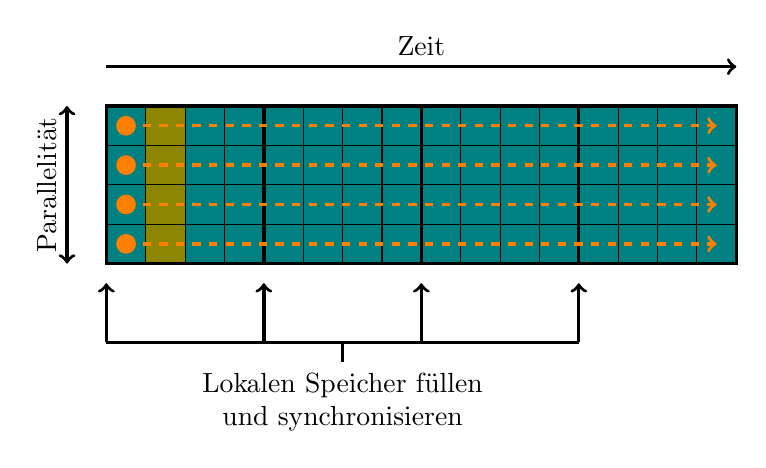
\begin{tikzpicture}
        % Farbe
        \fill [color = teal] (0.5, -0.5) rectangle (8.5, -2.5); % alles
        \fill [color = olive] (1.0, -0.5) rectangle (1.5, -2.5); % zweite Spalte

        % Rand
        \draw [line width = 1.2pt] (0.5, -0.5) rectangle (8.5, -2.5);

        % Zeilen
        \draw (0.5, -1.0) -- (8.5, -1.0); % Erste Zeile
        \draw (0.5, -1.5) -- (8.5, -1.5); % Zweite Zeile
        \draw (0.5, -2.0) -- (8.5, -2.0); % Dritte Zeile

        % Spalten
        \draw (1.0, -0.5) -- (1.0, -2.5); % Erste Spalte  (1. Q)
        \draw (1.5, -0.5) -- (1.5, -2.5); % Zweite Spalte (1. Q)
        \draw (2.0, -0.5) -- (2.0, -2.5); % Dritte Spalte (1. Q)

        \draw [line width = 1.2pt] (2.5, -0.5) -- (2.5, -2.5); % Sync #1
        
        \draw (3.0, -0.5) -- (3.0, -2.5); % Erste Spalte  (2. Q)
        \draw (3.5, -0.5) -- (3.5, -2.5); % Zweite Spalte (2. Q)
        \draw (4.0, -0.5) -- (4.0, -2.5); % Dritte Spalte (2. Q)

        \draw [line width = 1.2pt] (4.5, -0.5) -- (4.5, -2.5); % Sync #2

        \draw (5.0, -0.5) -- (5.0, -2.5); % Erste Spalte  (3. Q)
        \draw (5.5, -0.5) -- (5.5, -2.5); % Zweite Spalte (3. Q)
        \draw (6.0, -0.5) -- (6.0, -2.5); % Dritte Spalte (3. Q)

        \draw [line width = 1.2pt] (6.5, -0.5) -- (6.5, -2.5); % Sync #3

        \draw (7.0, -0.5) -- (7.0, -2.5); % Erste Spalte  (4. Q)
        \draw (7.5, -0.5) -- (7.5, -2.5); % Zweite Spalte (4. Q)
        \draw (8.0, -0.5) -- (8.0, -2.5); % Dritte Spalte (4. Q)

        % Spalten

        % Pfeil - erste Zeile
        \draw [->, dashed, line width = 1.2pt, draw = orange]
              (0.75, -0.75) -- (8.25, -0.75);
        \fill [color = orange] (0.75, -0.75) circle [radius = 0.125];

        % Pfeil - zweite Zeile
        \draw [->, dashed, line width = 1.2pt, draw = orange]
              (0.75, -1.25) -- (8.25, -1.25);
        \fill [color = orange] (0.75, -1.25) circle [radius = 0.125];

        % Pfeil - erste Zeile
        \draw [->, dashed, line width = 1.2pt, draw = orange]
              (0.75, -1.75) -- (8.25, -1.75);
        \fill [color = orange] (0.75, -1.75) circle [radius = 0.125];

        % Pfeil - erste Zeile
        \draw [->, dashed, line width = 1.2pt, draw = orange]
              (0.75, -2.25) -- (8.25, -2.25);
        \fill [color = orange] (0.75, -2.25) circle [radius = 0.125];

        % Beschriftung oben
        \draw [->, line width = 1.2pt] (0.5, 0.0) -- (8.5, 0.0)
              node [pos = 0.5, align = center, above] {Zeit};

        % Beschriftung links
        \draw [<->, line width = 1.2pt]
              (0.0, -2.5) -- (0.0, -0.5)
              node[pos = 0.5, align = center, above, sloped] {Parallelität};

        % Beschriftung unten
        \draw [line width = 1.2pt] (0.5, -3.5) -- (6.5, -3.5);
        \draw [->, line width = 1.2pt] (0.5, -3.5) -- (0.5, -2.75);
        \draw [->, line width = 1.2pt] (2.5, -3.5) -- (2.5, -2.75);
        \draw [->, line width = 1.2pt] (4.5, -3.5) -- (4.5, -2.75);
        \draw [->, line width = 1.2pt] (6.5, -3.5) -- (6.5, -2.75);
        \draw [line width = 1.2pt] (3.5, -3.5) -- (3.5, -3.75)
              node [pos = 1.0, align = center, below] {Lokalen Speicher füllen\\
              und synchronisieren};
    \end{tikzpicture}
    \caption{Berechnungen einer Arbeitsgruppe}
    \label{methoden:nbody:gpu:tilecluster}
\end{figure}

Quelltext~\ref{methoden:nbody:gpu:calcforces} zeigt den Pseudo-Code, der diese
Berechnung für GPUs umsetzt. Die Parameter \texttt{x} und \texttt{a} sind
Zeiger auf den globalen Speicher und enthalten die Positionen (\texttt{x}) und
Beschleunigungen (\texttt{a}) der Körper. Die Iteration über die Kacheln
erfordert zwei Synchronisierungspunkte. Der Erste stellt sicher, dass alle
Felder des lokalen Speichers befüllt wurden, bevor die Berechnung beginnt. Der
zweite Synchronisationspunkt garantiert, dass alle Berechnungen abgeschlossen
wurden, bevor die nächste Kachel verarbeitet wird.

\begin{code}
    \begin{minted}[breaklines,breakafter=\,,escapeinside=||,fontsize=\small]
          {c++}
void tile_calculation(float4* x, float3* a)
{
    |\textbf{\textcolor{keyword-green}{local}}| float4 sh_position[p];

    float3 acc = {0.0, 0.0, 0.0};
    int global_id = |\textbf{\textcolor{keyword-green}{group\_idx}}| * |\textbf{\textcolor{keyword-green}{group\_dim}}| + |\textbf{\textcolor{keyword-green}{unit\_idx}}|;

    float4 my_position = x[global_id];

    for(int i = 0, tile = 0; i < N; i += p, ++tile)
    {
        int idx = tile * |\textbf{\textcolor{keyword-green}{group\_dim}}| + |\textbf{\textcolor{keyword-green}{unit\_idx}}|;
        sh_position[|\textbf{\textcolor{keyword-green}{unit\_idx}}|] = x[idx];
        |\textbf{\textcolor{keyword-green}{synchronize}}|();

        acc = tile_calculation(my_position, acc);
        |\textbf{\textcolor{keyword-green}{synchronize}}|();
    }

    // Ergebnis für folgenden Integrationsschritt abspeichern
    a[global_id] = acc;
}
    \end{minted}
    \caption{Berechnung aller $N$ Interaktionen für $p$ Körper innerhalb einer
             Arbeitsgruppe mit $p$ Arbeitseinheiten}
    \label{methoden:nbody:gpu:calcforces}
\end{code}

Der gezeigte Pseudo-Code berechnet die Beschleunigung von $p$ Körpern eines
Systems, die durch ihre Interaktion mit allen $N$ Körpern im System
hervorgerufen wird. Um die Beschleunigung aller $N$ Körper zu berechnen, werden
mehrere Arbeitsgruppen eingesetzt. Da es $p$ Arbeitseinheiten pro Arbeitsgruppe
und eine Arbeitseinheit pro Körper gibt, ist die Zahl der benötigten
Arbeitsgruppen $\frac{N}{p}$. Im Gesamtsystem gibt es somit $N$
Arbeitseinheiten, die jeweils $N$ Berechnungen durchführen. Insgesamt werden
auf diese Weise $N^2$ Interaktionen berechnet. Eine Visualisierung dieses
Vorgangs findet sich in Abbildung~\ref{methoden:nbody:gpu:grid}. Die vertikale
Dimension zeigt die Parallelisierung, die durch $\frac{N}{p}$ unabhängige
Arbeitsgruppen mit jeweils $p$ Arbeitseinheiten erreicht wird. Die horizontale
Dimension zeigt die sequentielle Verarbeitung von $N$ Berechnungen durch jede
Arbeitseinheit. Eine Arbeitsgruppe lädt ihren lokalen Speicher alle $p$ Schritte
neu, um $p$ Positionen zu teilen.

\begin{figure}[htb]
    \centering
    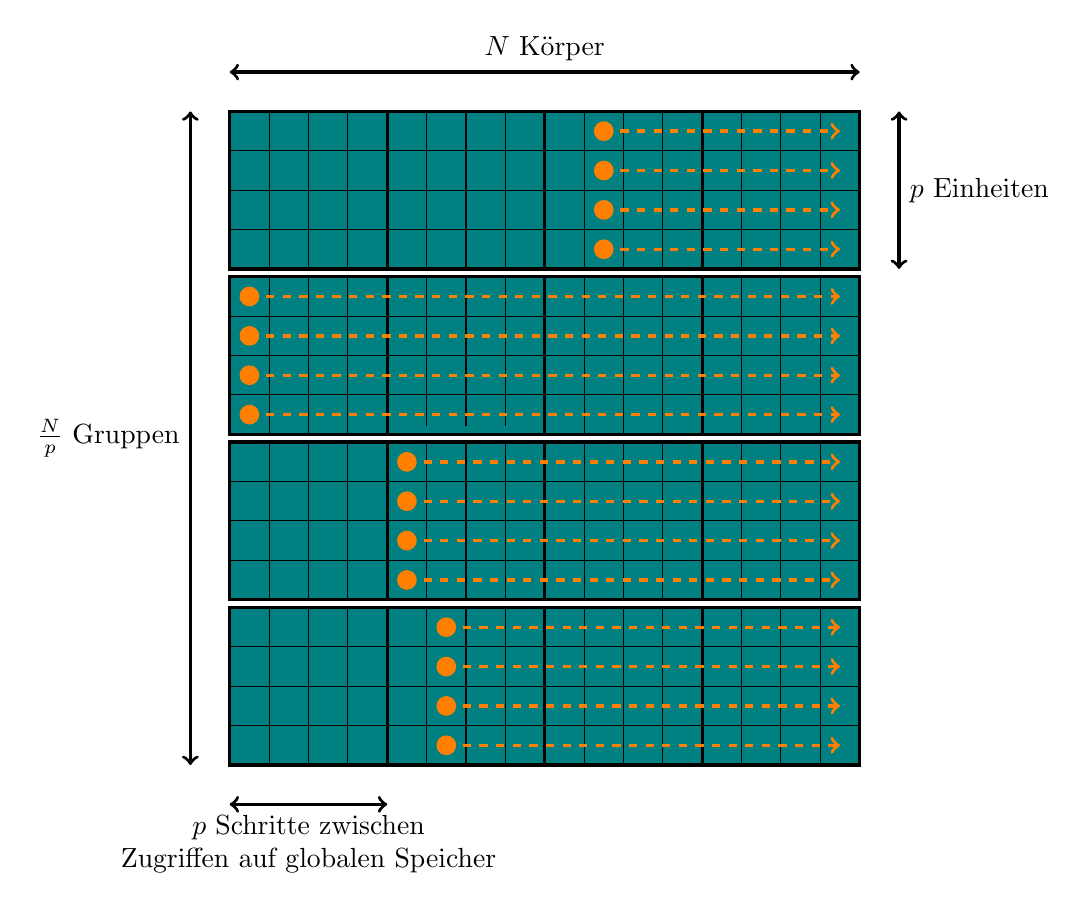
\begin{tikzpicture}
        %
        % ERSTE GRUPPE
        %

        % Farbe
        \fill [color = teal] (0.5, -0.5) rectangle (8.5, -2.5); % alles

        % Rand
        \draw [line width = 1.2pt] (0.5, -0.5) rectangle (8.5, -2.5);

        % Zeilen
        \draw (0.5, -1.0) -- (8.5, -1.0); % Erste Zeile
        \draw (0.5, -1.5) -- (8.5, -1.5); % Zweite Zeile
        \draw (0.5, -2.0) -- (8.5, -2.0); % Dritte Zeile

        % Spalten
        \draw (1.0, -0.5) -- (1.0, -2.5); % Erste Spalte  (1. Q)
        \draw (1.5, -0.5) -- (1.5, -2.5); % Zweite Spalte (1. Q)
        \draw (2.0, -0.5) -- (2.0, -2.5); % Dritte Spalte (1. Q)

        \draw [line width = 1.2pt] (2.5, -0.5) -- (2.5, -2.5); % Sync #1
        
        \draw (3.0, -0.5) -- (3.0, -2.5); % Erste Spalte  (2. Q)
        \draw (3.5, -0.5) -- (3.5, -2.5); % Zweite Spalte (2. Q)
        \draw (4.0, -0.5) -- (4.0, -2.5); % Dritte Spalte (2. Q)

        \draw [line width = 1.2pt] (4.5, -0.5) -- (4.5, -2.5); % Sync #2

        \draw (5.0, -0.5) -- (5.0, -2.5); % Erste Spalte  (3. Q)
        \draw (5.5, -0.5) -- (5.5, -2.5); % Zweite Spalte (3. Q)
        \draw (6.0, -0.5) -- (6.0, -2.5); % Dritte Spalte (3. Q)

        \draw [line width = 1.2pt] (6.5, -0.5) -- (6.5, -2.5); % Sync #3

        \draw (7.0, -0.5) -- (7.0, -2.5); % Erste Spalte  (4. Q)
        \draw (7.5, -0.5) -- (7.5, -2.5); % Zweite Spalte (4. Q)
        \draw (8.0, -0.5) -- (8.0, -2.5); % Dritte Spalte (4. Q)

        % Pfeil - erste Zeile
        \draw [->, dashed, line width = 1.2pt, draw = orange]
              (5.25, -0.75) -- (8.25, -0.75);
        \fill [color = orange] (5.25, -0.75) circle [radius = 0.125];

        % Pfeil - zweite Zeile
        \draw [->, dashed, line width = 1.2pt, draw = orange]
              (5.25, -1.25) -- (8.25, -1.25);
        \fill [color = orange] (5.25, -1.25) circle [radius = 0.125];

        % Pfeil - dritte Zeile
        \draw [->, dashed, line width = 1.2pt, draw = orange]
              (5.25, -1.75) -- (8.25, -1.75);
        \fill [color = orange] (5.25, -1.75) circle [radius = 0.125];

        % Pfeil - vierte Zeile
        \draw [->, dashed, line width = 1.2pt, draw = orange]
              (5.25, -2.25) -- (8.25, -2.25);
        \fill [color = orange] (5.25, -2.25) circle [radius = 0.125];

        %
        % ZWEITE GRUPPE
        %

        % Farbe
        \fill [color = teal] (0.5, -2.6) rectangle (8.5, -4.6);

        % Rand
        \draw [line width = 1.2pt] (0.5, -2.6) rectangle (8.5, -4.6);

        % Zeilen
        \draw (0.5, -3.1) -- (8.5, -3.1); % Erste Zeile
        \draw (0.5, -3.6) -- (8.5, -3.6); % Zweite Zeile
        \draw (0.5, -4.1) -- (8.5, -4.1); % Dritte Zeile

        % Spalten
        \draw (1.0, -2.6) -- (1.0, -4.6); % Erste Spalte  (1. Q)
        \draw (1.5, -2.6) -- (1.5, -4.6); % Zweite Spalte (1. Q)
        \draw (2.0, -2.6) -- (2.0, -4.6); % Dritte Spalte (1. Q)

        \draw [line width = 1.2pt] (2.5, -2.6) -- (2.5, -4.6); % Sync #1
        
        \draw (3.0, -2.6) -- (3.0, -4.5); % Erste Spalte  (2. Q)
        \draw (3.5, -2.6) -- (3.5, -4.5); % Zweite Spalte (2. Q)
        \draw (4.0, -2.6) -- (4.0, -4.5); % Dritte Spalte (2. Q)

        \draw [line width = 1.2pt] (4.5, -2.6) -- (4.5, -4.6); % Sync #2

        \draw (5.0, -2.6) -- (5.0, -4.6); % Erste Spalte  (3. Q)
        \draw (5.5, -2.6) -- (5.5, -4.6); % Zweite Spalte (3. Q)
        \draw (6.0, -2.6) -- (6.0, -4.6); % Dritte Spalte (3. Q)

        \draw [line width = 1.2pt] (6.5, -2.6) -- (6.5, -4.6); % Sync #3

        \draw (7.0, -2.6) -- (7.0, -4.6); % Erste Spalte  (4. Q)
        \draw (7.5, -2.6) -- (7.5, -4.6); % Zweite Spalte (4. Q)
        \draw (8.0, -2.6) -- (8.0, -4.6); % Dritte Spalte (4. Q)

        % Pfeil - erste Zeile
        \draw [->, dashed, line width = 1.2pt, draw = orange]
              (0.75, -2.85) -- (8.25, -2.85);
        \fill [color = orange] (0.75, -2.85) circle [radius = 0.125];

        % Pfeil - zweite Zeile
        \draw [->, dashed, line width = 1.2pt, draw = orange]
              (0.75, -3.35) -- (8.25, -3.35);
        \fill [color = orange] (0.75, -3.35) circle [radius = 0.125];

        % Pfeil - dritte Zeile
        \draw [->, dashed, line width = 1.2pt, draw = orange]
              (0.75, -3.85) -- (8.25, -3.85);
        \fill [color = orange] (0.75, -3.85) circle [radius = 0.125];

        % Pfeil - vierte Zeile
        \draw [->, dashed, line width = 1.2pt, draw = orange]
              (0.75, -4.35) -- (8.25, -4.35);
        \fill [color = orange] (0.75, -4.35) circle [radius = 0.125];

        %
        % DRITTE GRUPPE
        %

        % Farbe
        \fill [color = teal] (0.5, -4.7) rectangle (8.5, -6.7);

        % Rand
        \draw [line width = 1.2pt] (0.5, -4.7) rectangle (8.5, -6.7);

        % Zeilen
        \draw (0.5, -5.2) -- (8.5, -5.2); % Erste Zeile
        \draw (0.5, -5.7) -- (8.5, -5.7); % Zweite Zeile
        \draw (0.5, -6.2) -- (8.5, -6.2); % Dritte Zeile

        % Spalten
        \draw (1.0, -4.7) -- (1.0, -6.7); % Erste Spalte  (1. Q)
        \draw (1.5, -4.7) -- (1.5, -6.7); % Zweite Spalte (1. Q)
        \draw (2.0, -4.7) -- (2.0, -6.7); % Dritte Spalte (1. Q)

        \draw [line width = 1.2pt] (2.5, -4.7) -- (2.5, -6.7); % Sync #1
        
        \draw (3.0, -4.7) -- (3.0, -6.7); % Erste Spalte  (2. Q)
        \draw (3.5, -4.7) -- (3.5, -6.7); % Zweite Spalte (2. Q)
        \draw (4.0, -4.7) -- (4.0, -6.7); % Dritte Spalte (2. Q)

        \draw [line width = 1.2pt] (4.5, -4.7) -- (4.5, -6.7); % Sync #2

        \draw (5.0, -4.7) -- (5.0, -6.7); % Erste Spalte  (3. Q)
        \draw (5.5, -4.7) -- (5.5, -6.7); % Zweite Spalte (3. Q)
        \draw (6.0, -4.7) -- (6.0, -6.7); % Dritte Spalte (3. Q)

        \draw [line width = 1.2pt] (6.5, -4.7) -- (6.5, -6.7); % Sync #3

        \draw (7.0, -4.7) -- (7.0, -6.7); % Erste Spalte  (4. Q)
        \draw (7.5, -4.7) -- (7.5, -6.7); % Zweite Spalte (4. Q)
        \draw (8.0, -4.7) -- (8.0, -6.7); % Dritte Spalte (4. Q)

        % Pfeil - erste Zeile
        \draw [->, dashed, line width = 1.2pt, draw = orange]
              (2.75, -4.95) -- (8.25, -4.95);
        \fill [color = orange] (2.75, -4.95) circle [radius = 0.125];

        % Pfeil - zweite Zeile
        \draw [->, dashed, line width = 1.2pt, draw = orange]
              (2.75, -5.45) -- (8.25, -5.45);
        \fill [color = orange] (2.75, -5.45) circle [radius = 0.125];

        % Pfeil - dritte Zeile
        \draw [->, dashed, line width = 1.2pt, draw = orange]
              (2.75, -5.95) -- (8.25, -5.95);
        \fill [color = orange] (2.75, -5.95) circle [radius = 0.125];

        % Pfeil - vierte Zeile
        \draw [->, dashed, line width = 1.2pt, draw = orange]
              (2.75, -6.45) -- (8.25, -6.45);
        \fill [color = orange] (2.75, -6.45) circle [radius = 0.125];

        %
        % VIERTE GRUPPE
        %

        % Farbe
        \fill [color = teal] (0.5, -6.8) rectangle (8.5, -8.8);

        % Rand
        \draw [line width = 1.2pt] (0.5, -6.8) rectangle (8.5, -8.8);

        % Zeilen
        \draw (0.5, -7.3) -- (8.5, -7.3); % Erste Zeile
        \draw (0.5, -7.8) -- (8.5, -7.8); % Zweite Zeile
        \draw (0.5, -8.3) -- (8.5, -8.3); % Dritte Zeile

        % Spalten
        \draw (1.0, -6.8) -- (1.0, -8.8); % Erste Spalte  (1. Q)
        \draw (1.5, -6.8) -- (1.5, -8.8); % Zweite Spalte (1. Q)
        \draw (2.0, -6.8) -- (2.0, -8.8); % Dritte Spalte (1. Q)

        \draw [line width = 1.2pt] (2.5, -6.8) -- (2.5, -8.8); % Sync #1
        
        \draw (3.0, -6.8) -- (3.0, -8.8); % Erste Spalte  (2. Q)
        \draw (3.5, -6.8) -- (3.5, -8.8); % Zweite Spalte (2. Q)
        \draw (4.0, -6.8) -- (4.0, -8.8); % Dritte Spalte (2. Q)

        \draw [line width = 1.2pt] (4.5, -6.8) -- (4.5, -8.8); % Sync #2

        \draw (5.0, -6.8) -- (5.0, -8.8); % Erste Spalte  (3. Q)
        \draw (5.5, -6.8) -- (5.5, -8.8); % Zweite Spalte (3. Q)
        \draw (6.0, -6.8) -- (6.0, -8.8); % Dritte Spalte (3. Q)

        \draw [line width = 1.2pt] (6.5, -6.8) -- (6.5, -8.8); % Sync #3

        \draw (7.0, -6.8) -- (7.0, -8.8); % Erste Spalte  (4. Q)
        \draw (7.5, -6.8) -- (7.5, -8.8); % Zweite Spalte (4. Q)
        \draw (8.0, -6.8) -- (8.0, -8.8); % Dritte Spalte (4. Q)

        % Pfeil - erste Zeile
        \draw [->, dashed, line width = 1.2pt, draw = orange]
              (3.25, -7.05) -- (8.25, -7.05);
        \fill [color = orange] (3.25, -7.05) circle [radius = 0.125];

        % Pfeil - zweite Zeile
        \draw [->, dashed, line width = 1.2pt, draw = orange]
              (3.25, -7.55) -- (8.25, -7.55);
        \fill [color = orange] (3.25, -7.55) circle [radius = 0.125];

        % Pfeil - dritte Zeile
        \draw [->, dashed, line width = 1.2pt, draw = orange]
              (3.25, -8.05) -- (8.25, -8.05);
        \fill [color = orange] (3.25, -8.05) circle [radius = 0.125];

        % Pfeil - vierte Zeile
        \draw [->, dashed, line width = 1.2pt, draw = orange]
              (3.25, -8.55) -- (8.25, -8.55);
        \fill [color = orange] (3.25, -8.55) circle [radius = 0.125];

        % Beschriftung oben
        \draw [<->, line width = 1.2pt] (0.5, 0.0) -- (8.5, 0.0)
              node [pos = 0.5, align = center, above] {$N$ Körper};

        % Beschriftung links
        \draw [<->, line width = 1.2pt]
              (0.0, -8.8) -- (0.0, -0.5)
              node[pos = 0.5, left] {$\frac{N}{p}$ Gruppen};

        % Beschriftung unten
        \draw [<->, line width = 1.2pt]
              (0.5, -9.3) -- (2.5, -9.3)
              node[pos = 0.5, below, align = center]
              {$p$ Schritte zwischen\\Zugriffen auf globalen Speicher};

        % Beschriftung rechts
        \draw [<->, line width = 1.2pt]
              (9.0, -0.5) -- (9.0, -2.5)
              node[pos = 0.5, right] {$p$ Einheiten};
    \end{tikzpicture}
    \caption{Berechnung aller Interaktionen}
    \label{methoden:nbody:gpu:grid}
\end{figure}

%\section{Ergebnisse}
\label{ergebnisse}

\subsection{Erkennungsrate}
\label{ergebnisse:erfolg}

Für die Bestimmung der Erkennungsrate der \textit{Inferenz} werden in den folgenden Abschnitten zwei \textit{Scores}
gebildet: der \textit{Wordscore} $W$ und der \textit{Charscore} $C$. $W$ ist ein binärer Wert und gibt an, ob ein ganzes
Wort korrekt erkannt wurde. $C$ errechnet sich aus der Anzahl der korrekt erkannten Buchstaben geteilt durch die
Gesamtzahl der Buchstaben des Wortes. Anders ausgedrückt bedeutet $W = 1$ immer $C = 1$; $C < 1$ impliziert immer
$W = 0$.

Beispiele:

\begin{itemize}
    \item Der Text \glqq Bramel\grqq\ wird korrekt als \glqq Bramel\grqq\ erkannt. $W = C = 1$
    \item Der Text \glqq Ta\textbf{\color{red}n}nen\grqq\ wird als \glqq Ta\textbf{\color{red}u}nen\grqq\ erkannt.
          $W = 0$, $C = 0,8333$
\end{itemize}

Dieses Verfahren erlaubt eine grobe statistische Auswertung des Lernerfolgs, berücksichtigt jedoch einige Sonderfälle
nicht.

Beispiel:

\begin{itemize}
    \item Der Text \glqq Wehdel\grqq\ wird als \glqq NWehdel\grqq\ erkannt. $W = C = 0$
\end{itemize}

Obwohl der Text \glqq Wehdel\grqq\ in Gänze richtig erkannt wurde, sorgt das falsch erkannte \glqq N\grqq\ am
Wortbeginn für einen \textit{Wordscore} von 0. Da der \textit{Charscore} nur Buchstaben an ihrem korrekten Platz
berücksichtigt, diese jedoch durch das \glqq N\grqq\ um eine Position nach rechts verschoben wurden, ist er in diesem
Beispiel ebenfalls 0.

\subsection{\textit{Overfitting}}
\label{ergebnisse:overfitting}

Ein generelles Problem des maschinellen Lernens im Allgemeinen sowie der \gls{ctc}-Methode im Besonderen
(vgl.~\cite{graves2006}, S.\ 376) ist die Frage, wie eine zu große Abhängigkeit des Netzwerks von den
\textit{Trainings}-Daten vermieden werden kann. Diese \textit{Overfitting} genannte Sichtverengung des Netzwerks sorgt
zwar für exzellente Ergebnisse, wenn die \textit{Inferenz} auf den \textit{Trainings}-Daten durchgeführt wird,
verschlechtert jedoch die Erkennungsrate für unbekannte Daten.

Das im Rahmen dieser Arbeit entwickelte Netzwerk ist vor allem bei der Verwendung kleiner \textit{Trainings}-Datensätze
von \textit{Overfitting} betroffen, wie die in der Abbildung~\ref{ergebnisse:overfitting:messung} dargestellten
Messergebnisse zeigen. Als \textit{Trainings}-Grundlage dienen hier Datensätze mit \num{1000} bzw.\ \num{10000} Bildern,
der Loss sowie der Validierungs-Loss wurden automatisch durch \textit{Keras} ermittelt. In beiden Fällen ist anhand des
zunächst fallenden, dann steigenden Validierungs-Loss zu erkennen, dass das Netzwerk schon nach wenigen Epochen zu
\textit{Overfitting} neigt. Im weiteren Verlauf wurde daher nur mit Datensatzgrößen von mehr als \num{100000} Bildern
gearbeitet (siehe Abschnitt~\ref{ergebnisse:daten}).

\begin{figure}
    \centering
    \begin{tikzpicture}
        \begin{axis}[
            title = {Loss-Entwicklung für \num{1000} Bilder},
            xlabel = {Epochen},
            ylabel = {Loss},
            xmin = 0, xmax = 24,
            ymin = 0, ymax = 36,
            xtick = {0, 3, 6, 9, 12, 15, 18, 21, 24},
            ytick = {0, 6, 12, 18, 24, 30, 36},
            ymajorgrids = true,
            xmajorgrids = true,
            grid style = dashed,
            legend pos = south west,
            no markers
        ]

                \addplot table [x = epoch, y = loss, col sep = semicolon]{loss_1000.csv};
                \addlegendentry{loss};

                \addplot table [x = epoch, y = val_loss, col sep = semicolon]{loss_1000.csv};    
                \addlegendentry{val\_loss};
        \end{axis}
    \end{tikzpicture}

    \begin{tikzpicture}
        \begin{axis}[
            title = {Loss-Entwicklung für \num{10000} Bilder},
            xlabel = {Epochen},
            ylabel = {Loss},
            xmin = 0, xmax = 24,
            ymin = 0, ymax = 30,
            xtick = {0, 3, 6, 9, 12, 15, 18, 21, 24},
            ytick = {0, 6, 12, 18, 24, 30},
            ymajorgrids = true,
            xmajorgrids = true,
            grid style = dashed,
            legend pos = south west,
            no markers
        ]

                \addplot table [x = epoch, y = loss, col sep = semicolon]{loss_10k.csv};
                \addlegendentry{loss};

                \addplot table [x = epoch, y = val_loss, col sep = semicolon]{loss_10k.csv};    
                \addlegendentry{val\_loss};
        \end{axis}
    \end{tikzpicture}
    \caption{Loss und Genauigkeit für das Training mit kleinen Datensätzen\label{ergebnisse:overfitting:messung}}
\end{figure}

\subsection{Trainings- und Validierungsdaten}
\label{ergebnisse:daten}

Für das \textit{Training} wurden insgesamt zwei verschiedene Datensätze verwendet, die mit dem Präfix \texttt{wl6}
versehen sind. Die \texttt{wl6}-Datensätze werden für das Training eines Netzwerks für Texte mit fixer Wortlänge (sechs
Buchstaben) verwendet und enthalten Bilder zufälliger Größe (vgl.\ Tabelle~\ref{ergebnisse:daten:training}).

Die Validierung erfolgte durch \textit{Inferenz} in drei Schritten: zunächst auf dem Trainingsdatensatz, dann auf einem
generierten, vom Trainingsdatensatz verschiedenen Validierungsdatensatz und schließlich auf realen, aus dem vorliegenden
Kartenmaterial ausgeschnittenen Daten. Das Benennungsschema der künstlichen und realen Validierungsdatensätze entspricht
dem der \textit{Trainings}-Daten (vgl.\ Tabelle~\ref{ergebnisse:daten:validierung}).

\begin{table}
    \caption{Trainingsdatensätze}
    \centering
    \begin{tabular}{|c|c|c|c|c|}
        \hline
        \textbf{Name} & \textbf{Bildanzahl} & \textbf{Textlänge} & \textbf{Bildgröße} & \textbf{Datengröße}\\ \hline \hline
        \texttt{wl6\_120k} & \num{120164} & \num{6} & variabel & \SI{2,3357}{\gibi\byte} \\ \hline
        \texttt{wl6\_250k} & \num{250000} & \num{6} & variabel & \SI{4,8841}{\gibi\byte} \\ \hline
    \end{tabular}
    \label{ergebnisse:daten:training}
\end{table}

\begin{table}
    \caption{Validierungsdatensätze}
    \centering
    \begin{tabular}{|c|c|c|c|c|c|}
        \hline
        \textbf{Name} & \textbf{Typ} & \textbf{Bildanzahl} & \textbf{Textlänge} & \textbf{Bildgröße} & \textbf{Datengröße}\\ \hline \hline
        \texttt{wl6\_1000} & generiert & \num{1000} & \num{6} & variabel & \SI{19,4173}{\mebi\byte} \\ \hline
        \texttt{wl6\_real} & real & \num{27} & \num{6} & variabel & \SI{549,5}{\kibi\byte} \\ \hline
    \end{tabular}
    \label{ergebnisse:daten:validierung}
\end{table}

\subsection{\textit{Scores}, \textit{Losses} und Genauigkeit}
\label{ergebnisse:scores}

Alle der im Folgenden präsentierten Ergebnisse wurden mit Netzwerken erzielt, die auf ihren jeweiligen Datensätzen über
25 Epochen \textit{trainiert} wurden.

Die in Tabelle~\ref{ergebnisse:scores:scores} (visualisiert in Abbildung~\ref{ergebnisse:scores:scoresviz}) für die fixe
Wortlänge von 6 ermittelten Ergebnisse zeigen, dass das Netzwerk von einer größeren Datenmenge profitiert. Durch den
Sprung vom Datensatz \texttt{wl6\_120k} auf \texttt{wl6\_250k} werden für alle Validierungsdatensätze deutlich bessere
Ergebnisse erzielt.

\begin{table}
    \caption{Scores}
    \centering
    \begin{tabular}{|c|c|c|c|}
        \hline
        \textbf{Trainingsdatensatz} & \textbf{Validierungsdatensatz} & $\sum$ \textbf{Wordscore} / Gesamtzahl & \textbf{Charscore} ($\varnothing$)\\ \hline \hline
        \texttt{wl6\_120k} & \texttt{wl6\_120k} & \num{80824/120164} & \num{0,6819} \\ \hline
        \texttt{wl6\_120k} & \texttt{wl6\_1000} & \num{661/1000} & \num{0,6685} \\ \hline
        \texttt{wl6\_120k} & \texttt{wl6\_real} & \num{1/27} & \num{0,3889} \\ \hline
        \texttt{wl6\_250k} & \texttt{wl6\_250k} & \num{226432/250000} & \num{0,9086} \\ \hline 
        \texttt{wl6\_250k} & \texttt{wl6\_1000} & \num{759/1000} & \num{0,8630} \\ \hline 
        \texttt{wl6\_250k} & \texttt{wl6\_real} & \num{4/27} & \num{0,4753} \\ \hline \hline 
    \end{tabular}
    \label{ergebnisse:scores:scores}
\end{table}

\begin{figure}
    \centering
    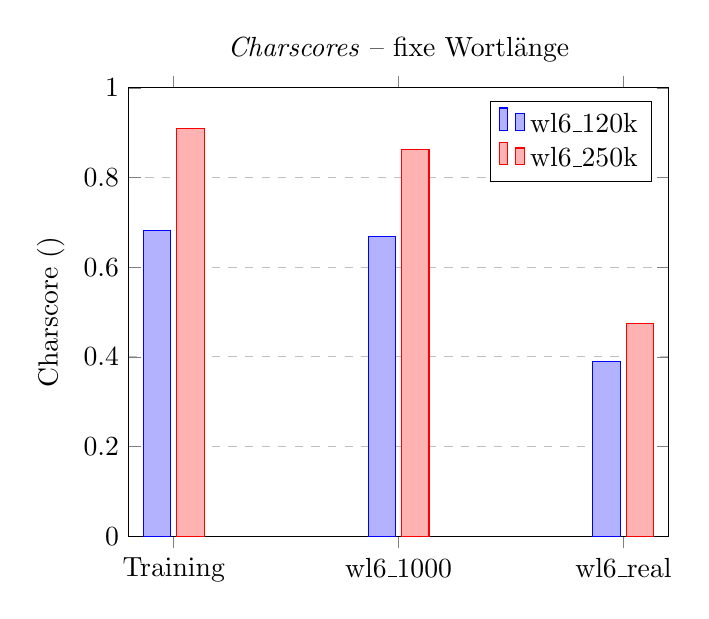
\begin{tikzpicture}
        \begin{axis}[
            title = {\textit{Charscores} -- fixe Wortlänge},
            ylabel = {Charscore ($\varnothing$)},
            ymin = 0, ymax = 1,
            ytick = {0, 0.2, 0.4, 0.6, 0.8, 1},
            ymajorgrids = true,
            grid style = dashed,
            legend pos = north east,
            symbolic x coords = {Training, wl6\_1000, wl6\_real},
            xtick = data,
            ybar
        ]

            \addplot coordinates {(Training, 0.6819) (wl6\_1000, 0.6685) (wl6\_real, 0.3889)};
            \addlegendentry{wl6\_120k};

            \addplot coordinates {(Training, 0.9086) (wl6\_1000, 0.863) (wl6\_real, 0.4753)};
            \addlegendentry{wl6\_250k};
        \end{axis}
    \end{tikzpicture}
    \caption{Charscores für verschiedene \textit{Trainings}-Datensatzgrößen\label{ergebnisse:scores:scoresviz}}
\end{figure}

\begin{figure}
    \centering
    \begin{tikzpicture}
        \begin{axis}[
            title = {Loss-Entwicklung für \texttt{wl6\_120k}},
            xlabel = {Epochen},
            ylabel = {Loss},
            xmin = 0, xmax = 24,
            ymin = 0, ymax = 11,
            xtick = {0, 3, 6, 9, 12, 15, 18, 21, 24},
            ytick = {0, 1, 2, 3, 4, 5, 6, 7, 8, 9, 10, 11},
            ymajorgrids = true,
            xmajorgrids = true,
            grid style = dashed,
            legend pos = north east,
            no markers
        ]

                \addplot table [x = epoch, y = loss, col sep = semicolon]{loss_120k.csv};
                \addlegendentry{loss};

                \addplot table [x = epoch, y = val_loss, col sep = semicolon]{loss_120k.csv};    
                \addlegendentry{val\_loss};
        \end{axis}
    \end{tikzpicture}

    \begin{tikzpicture}
        \begin{axis}[
            title = {Genauigkeitsentwicklung für \texttt{wl6\_120k}},
            xlabel = {Epochen},
            ylabel = {Genauigkeit},
            xmin = 0, xmax = 24,
            ymin = 0, ymax = 1.1,
            xtick = {0, 3, 6, 9, 12, 15, 18, 21, 24},
            ytick = {0, 0.1, 0.2, 0.3, 0.4, 0.5, 0.6, 0.7, 0.8, 0.9, 1},
            ymajorgrids = true,
            xmajorgrids = true,
            grid style = dashed,
            legend pos = south east,
            no markers
        ]

                \addplot table [x = epoch, y = acc, col sep = semicolon]{loss_120k.csv};
                \addlegendentry{acc};

                \addplot table [x = epoch, y = val_acc, col sep = semicolon]{loss_120k.csv};    
                \addlegendentry{val\_acc};
        \end{axis}
    \end{tikzpicture}
    \caption{Loss und Genauigkeit für den Datensatz \texttt{wl6\_120k}\label{ergebnisse:scores:loss120k}}
\end{figure}

\begin{figure}
    \centering
    \begin{tikzpicture}
        \begin{axis}[
            title = {Loss-Entwicklung für \texttt{wl6\_250k}},
            xlabel = {Epochen},
            ylabel = {Loss},
            xmin = 0, xmax = 24,
            ymin = 0, ymax = 9,
            xtick = {0, 3, 6, 9, 12, 15, 18, 21, 24},
            ytick = {0, 1, 2, 3, 4, 5, 6, 7, 8, 9},
            ymajorgrids = true,
            xmajorgrids = true,
            grid style = dashed,
            legend pos = north east,
            no markers
        ]

                \addplot table [x = epoch, y = loss, col sep = semicolon]{loss_250k.csv};
                \addlegendentry{loss};

                \addplot table [x = epoch, y = val_loss, col sep = semicolon]{loss_250k.csv};    
                \addlegendentry{val\_loss};
        \end{axis}
    \end{tikzpicture}

    \begin{tikzpicture}
        \begin{axis}[
            title = {Genauigkeitsentwicklung für \texttt{wl6\_250k}},
            xlabel = {Epochen},
            ylabel = {Genauigkeit},
            xmin = 0, xmax = 24,
            ymin = 0, ymax = 1.1,
            xtick = {0, 3, 6, 9, 12, 15, 18, 21, 24},
            ytick = {0, 0.1, 0.2, 0.3, 0.4, 0.5, 0.6, 0.7, 0.8, 0.9, 1},
            ymajorgrids = true,
            xmajorgrids = true,
            grid style = dashed,
            legend pos = south east,
            no markers
        ]

                \addplot table [x = epoch, y = acc, col sep = semicolon]{loss_250k.csv};
                \addlegendentry{acc};

                \addplot table [x = epoch, y = val_acc, col sep = semicolon]{loss_250k.csv};    
                \addlegendentry{val\_acc};
        \end{axis}
    \end{tikzpicture}
    \caption{Loss und Genauigkeit für den Datensatz \texttt{wl6\_250k}\label{ergebnisse:scores:loss250k}}
\end{figure}

\subsection{Performance}

Neben den erzielten Ergebnissen ist für die Nutzung auf einem HPC-System auch die Ausführungsgeschwindigkeit von
Interesse. Diese soll in den folgenden Abschnitten näher betrachtet werden.

\subsubsection{\textit{Training}}
\label{ergebnisse:performance:training}

Aufgrund der großen Datenmengen und der Komplexität des Netzwerks dauert das \textit{Training} -- abhängig vom konkreten
Datensatz -- wenige bis viele Stunden. Dabei zeigt sich, dass die Laufzeit proportional zur Größe des Datensatzes
ansteigt  (siehe Tabelle~\ref{ergebnisse:performance:training:laufzeit}).

\begin{table}
    \caption{\textit{Trainings}-Laufzeiten}
    \centering
    \begin{tabular}{|c|c|c|}
        \hline
        \textbf{Trainingsdatensatz} & \textbf{Gesamtlaufzeit} & \textbf{Epochenlaufzeit} \\ \hline \hline
        \texttt{wl6\_120k} & \SI{4}{\hour} \SI{20}{\minute} \SI{54}{\second} & \SI{10}{\min} \SI{39}{\second} \\ \hline
        \texttt{wl6\_250k} & \SI{9}{\hour} \SI{03}{\minute} \SI{22}{\second} & \SI{21}{\min} \SI{44}{\second} \\ \hline
    \end{tabular}
    \label{ergebnisse:performance:training:laufzeit}
\end{table}

\subsubsection{\textit{Inferenz}}

Bei der \textit{Inferenz} zeigt sich das gleiche Bild wie beim \textit{Training}. Auch hier steigt die Laufzeit
proportional zur Datenmenge an, fällt aber durch den geringeren Rechenaufwand deutlich kleiner aus als beim
\textit{Training} (siehe Tabelle~\ref{ergebnisse:performance:inferenz:laufzeit}).

\begin{table}[h]
    \caption{\textit{Inferenz}-Laufzeiten}
    \centering
    \begin{tabular}{|c|c|c|}
        \hline
        \textbf{Validierungsdatensatz} & \textbf{Gesamtlaufzeit} & \textbf{Laufzeit pro Bild}\\ \hline \hline
        \texttt{wl6\_120k} & \SI{19}{\minute} \SI{25}{\second} & \SI{9,7}{\milli\second} \\ \hline
        \texttt{wl6\_250k} & \SI{40}{\minute} \SI{17}{\second} & \SI{9,7}{\milli\second} \\ \hline
    \end{tabular}
    \label{ergebnisse:performance:inferenz:laufzeit}
\end{table}

%\include{bewertung}
%\section{Fazit}
\label{fazit}

\subsection{Ausblick}
\label{fazit:ausblick}

\begin{itemize}
    \item Rechtsstreit Oracle - Google -> Ende für HIP?
    \item SYCL auf FPGA
\end{itemize}

\subsection{Notizen}

Die vollständigen Quelltexte der Benchmarks sowie die \LaTeX-Quelltexte dieser
Arbeit sind öffentlich unter dem folgenden Link erreichbar:

\url{https://github.com/j-stephan/fpg}


\listoflistings

%\appendix

\section{CUDA-Kernel}

\subsection{zcopy}

\begin{code}
    \begin{minted}[breaklines,breakafter=\,,escapeinside=||,fontsize=\small]{cuda}
__global__ void read_write(const float4* __restrict__ A,
                                 float4* __restrict__ B,
                           std::size_t num_elems)
{
    auto stride = gridDim.x * blockDim.x;
    for(auto i = blockIdx.x * blockDim.x + threadIdx.x;
             i < elems;
             i += stride)
    {
        B[i] = A[i];
    }
}

__global__ void write(float4* __restrict__ B, std::size_t num_elems)
{
    auto stride = gridDim.x * blockDim.x;
    for(auto i = blockIdx.x * blockDim.x + threadIdx.x;
             i < elems;
             i += stride)
    {
        B[i] = make_float4{0.f, 0.f, 0.f, 0.f};
    }
}
    \end{minted}
    \caption{zcopy -- CUDA-Implementierung}
    \label{anhang:cuda:zcopy}
\end{code}

\subsection{Reduction}
\label{anhang:cuda:reduction}

\subsection{N-Body}

\section{HIP-Kernel}

\subsection{zcopy}

\begin{code}
    \begin{minted}[breaklines,breakafter=\,,escapeinside=||,fontsize=\small]{cuda}
__global__ void read_write(const float4* __restrict__ A,
                                 float4* __restrict__ B,
                           std::size_t num_elems)
{
    auto stride = |\textcolor{keyword-green}{hipGridDim\_x}| * |\textcolor{keyword-green}{hipBlockDim\_x}|;
        for(auto i = |\textcolor{keyword-green}{hipBlockIdx\_x}| * |\textcolor{keyword-green}{hipBlockDim\_x}| + |\textcolor{keyword-green}{hipThreadIdx\_x}|;
             i < elems;
             i += stride)
    {
        B[i] = A[i];
    }
}

__global__ void write(float4* __restrict__ B, std::size_t num_elems);
{
    auto stride = |\textcolor{keyword-green}{hipGridDim\_x}| * |\textcolor{keyword-green}{hipBlockDim\_x}|;
    for(auto i = |\textcolor{keyword-green}{hipBlockIdx\_x}| * |\textcolor{keyword-green}{hipBlockDim\_x}| + |\textcolor{keyword-green}{hipThreadIdx\_x}|;
             i < elems;
             i += stride)
    {
        B[i] = make_float4{0.f, 0.f, 0.f, 0.f};
    }
}
    \end{minted}
    \caption{zcopy -- HIP-Implementierung}
    \label{anhang:hip:zcopy}
\end{code}

\subsection{Reduction}
\label{anhang:hip:reduction}

\subsection{N-Body}

\begin{code}
    \begin{minted}[breaklines,breakafter=\,,escapeinside=||,fontsize=\small]{cuda}
|\textbf{\textcolor{keyword-green}{constexpr}}| auto eps = 0.001f;
|\textbf{\textcolor{keyword-green}{constexpr}}| auto eps2 = eps * eps;

__device__ auto body_body_interaction(float4 bi, float4 bj, float3 ai)
-> float3
{
    // r_ij [3 FLOPS]
    auto r = float3{};
    r.x = bj.x - bi.x;
    r.y = bj.y - bi.y;
    r.z = bj.z - bi.z;

    // dist_sqr = skalarprodukt(r_ij, r_ij) + epsilon^2 [6 FLOPS]
    auto dist_sqr = fmaf(r.x, r.x,
                         fmaf(r.y, r.y,
                              fmaf(r.z, r.z, eps2)));

    // inv_dist_cube = 1 / dist_sqr^(3/2) [4 FLOPS]
    auto dist_sixth = dist_sqr * dist_sqr * dist_sqr;
    auto inv_dist_cube = rsqrtf(dist_sixth);

    // s = m_j * inv_dist_cube [1 FLOP]
    auto s = bj.w * inv_dist_cube;

    // a_i = a_i + s * r_ij [6 FLOPS]
    ai.x = fmaf(r.x, s, ai.x);
    ai.y = fmaf(r.y, s, ai.y);
    ai.z = fmaf(r.z, s, ai.z);

    return ai;
}
    \end{minted}
    \caption{body\_body\_interaction - HIP-Implementierung}
    \label{anhang:hip:bodybodyinteraction}
\end{code}

\begin{code}
    \begin{minted}[breaklines,breakafter=\,,escapeinside=||,fontsize=\small]{cuda}
__device__ auto force_calculation(float4 body_pos,
                                  const float4* positions,
                                  unsigned tiles)
-> float3
{
    extern __shared__ float4 sh_position[];

    auto acc = float3{};

    for(auto tile = 0u; tile < tiles; ++tile)
    {
        auto idx = tile * |\textcolor{keyword-green}{hipBlockDim\_x}| + |\textcolor{keyword-green}{hipThreadIdx\_x}|;

        sh_position[|\textcolor{keyword-green}{hipThreadIdx\_x}|] = positions[idx];
        __syncthreads();

        // entspricht tile_calculation()
        #pragma unroll
        for(auto i = 0u; i < |\textcolor{keyword-green}{hipBlockDim\_x}|; ++i)
            acc = body_body_interaction(body_pos, sh_position[i],
                                        acc);
        __syncthreads();
    }
    return acc;
}
    \end{minted}
    \caption{force\_calculation - HIP-Implementierung}
    \label{anhang:hip:forcecalculation}
\end{code}


\section{HC-Kernel}

\subsection{zcopy}

\begin{code}
    \begin{minted}[breaklines,breakafter=\,,escapeinside=||,fontsize=\small]{c++}
[[hc]]
template <typename DataT>
void read_write(hc::tiled_index<1> idx, hc::array_view<DataT, 1> A,
                hc::array_view<DataT, 1> B, std::size_t elems,
                unsigned int tiles, unsigned int tile_size)
{
    auto stride = tiles * tile_size;
    for(auto i = idx.tile[0] * tile_size + idx.local[0];
             i < elems;
             i += stride)
    {
        B[i] = A[i];
    }
}

[[hc]]
template <typename DataT>
void write(hc::tiled_index<1> idx, hc::array_view<DataT, 1> B,
           std::size_t elems, unsigned int tiles,
           unsigned int tile_size)
{
    auto stride = tiles * tile_size;
    for(auto i = idx.tile[0] * tile_size + idx.local[0];
             i < elems;
             i += stride)
    {
        B[i] = DataT{};
    }
}
    \end{minted}
    \caption{zcopy - HC-Implementierung}
    \label{anhang:hc:zcopy}
\end{code}

\subsection{Reduction}
\label{anhang:hc:reduction}

\subsection{N-Body}

\begin{code}
    \begin{minted}[breaklines,breakafter=\,,escapeinside=||,fontsize=\small]{c++}
using float3 = hc::short_vector::float3;
using float4 = hc::short_vector::float4;

[[hc]]
auto body_body_interaction(float4 bi, float4 bj, float3 ai) -> float3
{
    constexpr auto eps = 0.001f;
    constexpr auto eps2 = eps * eps;

    // r_ij [3 FLOPS]
    auto r = bj.get_xyz() - bi.get_xyz();

    // dist_sqr = skalarprodukt(r, r) + epsilon^2 [6 FLOPS]
    auto dist_sqr = fmaf(r.x, r.x,
                         fmaf(r.y, r.y,
                              fmaf(r.z, r.z, eps2)));

    // inv_dist_cube = 1 / dist_sqr^(3/2) [4 FLOPS]
    auto dist_sixth = dist_sqr * dist_sqr * dist_sqr;
    auto inv_dist_cube = rsqrtf(dist_sixth);

    // s = m_j * inv_dist_cube [1 FLOP]

    // a_i = a_i + s * r_ij [6 FLOPS]
    ai.x = fmaf(r.x, s, ai.x);
    ai.y = fmaf(r.y, s, ai.y);
    ai.z = fmaf(r.z, s, ai.z);

    return ai;
}
    \end{minted}
    \caption{body\_body\_interaction - HC-Implementierung}
    \label{anhang:hc:bodybodyinteraction}
\end{code}

\begin{code}
    \begin{minted}[breaklines,breakafter=\,,escapeinside=||,fontsize=\small]{c++}
using float3 = hc::short_vector::float3;
using float4 = hc::short_vector::float4;

[[hc]]
auto force_calculation(hc::tiled_index<1> idx, float4 body_pos,
                       hc::array_view<const float4, 1> positions,
                       float4* sh_position, unsigned tiles)
-> float3
{
    auto acc = float3{};

    for(auto tile = 0u; tile < tiles; ++tile)
    {
        auto id = tile * idx.tile_dim[0] + idx.local[0];

        sh_position[idx.local[0]] = positions[id];
        idx.barrier.wait_with_tile_static_memory_fence();

        // entspricht tile_calculation()
        #pragma unroll
        for(auto i = 0u; i < idx.tile_dim[0]; ++i)
            acc = body_body_interaction(body_pos, sh_position[i],
                                        acc);
        idx.barrier.wait_with_tile_static_memory_fence();
    }
    return acc;
}
    \end{minted}
    \caption{force\_calculation - HC-Implementierung}
    \label{anhang:hc:forcecalculation}
\end{code}

\section{SYCL-Kernel}

\subsection{zcopy}

\begin{code}
    \begin{minted}[breaklines,breakafter=\,,escapeinside=||,fontsize=\small]{c++}
struct reader_writer
{
    cl::sycl::accessor<cl::sycl::float4, 1,
                       cl::sycl::access::mode::read,
                       cl::sycl::access::target::global_buffer> A;
    cl::sycl::accessor<cl::sycl::float4, 1,
                       cl::sycl::access::mode::discard_write,
                       cl::sycl::access::target::global_buffer> B;

    auto operator()(cl::sycl::nd_item<1> my_item) -> void
    {
        auto stride = my_item.get_group_range(0) *
                      my_item.get_local_range(0);
        for(auto i = my_item.get_global_id(0); i < elems; i += stride)
        {
            B[i] = A[i];
        }
    }
};

struct writer
{
    cl::sycl::accessor<cl::sycl::float4, 1,
                       cl::sycl::access::mode::discard_write,
                       cl::sycl::access::target::global_buffer> B;

    auto operator()(cl::sycl::nd_item<1> my_item) -> void
    {
        auto stride = my_item.get_group_range(0) *
                      my_item.get_local_range(0);
        for(auto i = my_item.get_global_id(0); i < elems; i += stride)
        {
            B[i] = cl::sycl::float4{};
        }
    }
};
    \end{minted}
    \caption{zcopy -- SYCL-Implementierung}
    \label{anhang:sycl:zcopy}
\end{code}

\subsection{Reduction}
\label{anhang:sycl:reduction}

\subsection{N-Body}

\section{Benchmark-Ergebnisse}

\subsection{HIP-zcopy (AMD)}
\label{anhang:hip:amdzcopyfig}

\begin{figure}[H]
    \centering
    \begin{tikzpicture}
        \begin{axis}[
            title = {zcopy -- Lesen + Schreiben -- Vega 64},
            xlabel = {Blöcke pro Multiprozessor},
            ylabel = {Bandbreite [\si{\gibi\byte\per\second}]},
            xmode = log,
            log basis x = 2,
            xmin = 1, xmax = 4096,
            xticklabel = {\xinttheiexpr2^\tick\relax},
            log ticks with fixed point,
            ymajorgrids = true,
            xmajorgrids = true,
            grid style = dashed,
            legend cell align = left,
            legend pos = south east,
            no markers,
            every axis plot/.append style = {very thick},
            width = 0.75\textwidth,
            scale only axis,
            cycle list name = exotic,
            /pgf/number format/.cd, use comma
        ]
            \addplot table [x = blocks_per_sm, y = throughput-64,
                            col sep = semicolon]
                           {data/zcopy-amd-hip-vega64-rw.csv};
            \addlegendentry{$\text{Blockgröße} = 64$} 

            \addplot table [x = blocks_per_sm, y = throughput-128,
                            col sep = semicolon]
                           {data/zcopy-amd-hip-vega64-rw.csv};
            \addlegendentry{$\text{Blockgröße} = 128$} 

            \addplot table [x = blocks_per_sm, y = throughput-256,
                            col sep = semicolon]
                           {data/zcopy-amd-hip-vega64-rw.csv};
            \addlegendentry{$\text{Blockgröße} = 256$} 

            \addplot table [x = blocks_per_sm, y = throughput-512,
                            col sep = semicolon]
                           {data/zcopy-amd-hip-vega64-rw.csv};
            \addlegendentry{$\text{Blockgröße} = 512$} 

            \addplot table [x = blocks_per_sm, y = throughput-1024,
                            col sep = semicolon]
                           {data/zcopy-amd-hip-vega64-rw.csv};
            \addlegendentry{$\text{Blockgröße} = 1024$} 
        \end{axis}
    \end{tikzpicture}
    \caption{Bandbreite der Vega 64 (Lesen und Schreiben, HIP)}
\end{figure}

\begin{figure}[H]
    \centering
    \begin{tikzpicture}
        \begin{axis}[
            title = {zcopy -- Schreiben -- Vega 64},
            xlabel = {Blöcke pro Multiprozessor},
            ylabel = {Bandbreite [\si{\gibi\byte\per\second}]},
            xmode = log,
            log basis x = 2,
            xmin = 1, xmax = 4096,
            xticklabel = {\xinttheiexpr2^\tick\relax},
            log ticks with fixed point,
            ymajorgrids = true,
            xmajorgrids = true,
            grid style = dashed,
            legend cell align = left,
            legend pos = south east,
            no markers,
            every axis plot/.append style = {very thick},
            width = 0.75\textwidth,
            scale only axis,
            cycle list name = exotic,
            /pgf/number format/.cd, use comma
        ]
            \addplot table [x = blocks_per_sm, y = throughput-64,
                            col sep = semicolon]
                           {data/zcopy-amd-hip-vega64-w.csv};
            \addlegendentry{$\text{Blockgröße} = 64$} 

            \addplot table [x = blocks_per_sm, y = throughput-128,
                            col sep = semicolon]
                           {data/zcopy-amd-hip-vega64-w.csv};
            \addlegendentry{$\text{Blockgröße} = 128$} 

            \addplot table [x = blocks_per_sm, y = throughput-256,
                            col sep = semicolon]
                           {data/zcopy-amd-hip-vega64-w.csv};
            \addlegendentry{$\text{Blockgröße} = 256$} 

            \addplot table [x = blocks_per_sm, y = throughput-512,
                            col sep = semicolon]
                           {data/zcopy-amd-hip-vega64-w.csv};
            \addlegendentry{$\text{Blockgröße} = 512$} 

            \addplot table [x = blocks_per_sm, y = throughput-1024,
                            col sep = semicolon]
                           {data/zcopy-amd-hip-vega64-w.csv};
            \addlegendentry{$\text{Blockgröße} = 1024$} 
        \end{axis}
    \end{tikzpicture}
    \caption{Bandbreite der Vega 64 (Schreiben, HIP)}
\end{figure}

\subsection{HIP-zcopy (NVIDIA)}
\label{anhang:hip:nvzcopyfig}

\begin{figure}[H]
    \centering
    \begin{tikzpicture}
        \begin{axis}[
            title = {zcopy -- Lesen + Schreiben -- generisch -- K20x},
            xlabel = {Blöcke pro Multiprozessor},
            ylabel = {Bandbreite [\si{\gibi\byte\per\second}]},
            xmode = log,
            log basis x = 2,
            xmin = 1, xmax = 8192,
            ymin = 40, ymax = 190,
            xticklabel = {\xinttheiexpr2^\tick\relax},
            log ticks with fixed point,
            ymajorgrids = true,
            xmajorgrids = true,
            grid style = dashed,
            legend cell align = left,
            legend pos = south east,
            no markers,
            every axis plot/.append style = {very thick},
            width = 0.75\textwidth,
            scale only axis,
            cycle list name = exotic,
            /pgf/number format/.cd, use comma
        ]
            \addplot table [x = blocks_per_sm, y = throughput-64,
                            col sep = semicolon]
                           {data/zcopy-nvidia-hip-k20x-generic-rw.csv};
            \addlegendentry{$\text{Blockgröße} = 64$} 

            \addplot table [x = blocks_per_sm, y = throughput-128,
                            col sep = semicolon]
                           {data/zcopy-nvidia-hip-k20x-generic-rw.csv};
            \addlegendentry{$\text{Blockgröße} = 128$} 

            \addplot table [x = blocks_per_sm, y = throughput-256,
                            col sep = semicolon]
                           {data/zcopy-nvidia-hip-k20x-generic-rw.csv};
            \addlegendentry{$\text{Blockgröße} = 256$} 

            \addplot table [x = blocks_per_sm, y = throughput-512,
                            col sep = semicolon]
                           {data/zcopy-nvidia-hip-k20x-generic-rw.csv};
            \addlegendentry{$\text{Blockgröße} = 512$} 

            \addplot table [x = blocks_per_sm, y = throughput-1024,
                            col sep = semicolon]
                           {data/zcopy-nvidia-hip-k20x-generic-rw.csv};
            \addlegendentry{$\text{Blockgröße} = 1024$} 
        \end{axis}
    \end{tikzpicture}
    \caption{K20x-Bandbreite für generische Blöcke (Lesen und Schreiben, HIP)}
\end{figure}

\begin{figure}[H]
    \centering
    \begin{tikzpicture}
        \begin{axis}[
            title = {zcopy -- Schreiben -- generisch -- K20x},
            xlabel = {Blöcke pro Multiprozessor},
            ylabel = {Bandbreite [\si{\gibi\byte\per\second}]},
            xmode = log,
            log basis x = 2,
            xmin = 1, xmax = 8192,
            ymin = 70, ymax = 190,
            xticklabel = {\xinttheiexpr2^\tick\relax},
            log ticks with fixed point,
            ymajorgrids = true,
            xmajorgrids = true,
            grid style = dashed,
            legend cell align = left,
            legend pos = south east,
            no markers,
            every axis plot/.append style = {very thick},
            width = 0.75\textwidth,
            scale only axis,
            cycle list name = exotic,
            /pgf/number format/.cd, use comma
        ]
            \addplot table [x = blocks_per_sm, y = throughput-64,
                            col sep = semicolon]
                           {data/zcopy-nvidia-hip-k20x-generic-w.csv};
            \addlegendentry{$\text{Blockgröße} = 64$} 

            \addplot table [x = blocks_per_sm, y = throughput-128,
                            col sep = semicolon]
                           {data/zcopy-nvidia-hip-k20x-generic-w.csv};
            \addlegendentry{$\text{Blockgröße} = 128$} 

            \addplot table [x = blocks_per_sm, y = throughput-256,
                            col sep = semicolon]
                           {data/zcopy-nvidia-hip-k20x-generic-w.csv};
            \addlegendentry{$\text{Blockgröße} = 256$} 

            \addplot table [x = blocks_per_sm, y = throughput-512,
                            col sep = semicolon]
                           {data/zcopy-nvidia-hip-k20x-generic-w.csv};
            \addlegendentry{$\text{Blockgröße} = 512$} 

            \addplot table [x = blocks_per_sm, y = throughput-1024,
                            col sep = semicolon]
                           {data/zcopy-nvidia-hip-k20x-generic-w.csv};
            \addlegendentry{$\text{Blockgröße} = 1024$} 
        \end{axis}
    \end{tikzpicture}
    \caption{K20x-Bandbreite für generische Blöcke (Schreiben, HIP)}
\end{figure}

\begin{figure}[H]
    \centering
    \begin{tikzpicture}
        \begin{axis}[
            title = {zcopy -- Lesen + Schreiben -- optimiert -- K20x},
            xlabel = {Blöcke pro Multiprozessor},
            ylabel = {Bandbreite [\si{\gibi\byte\per\second}]},
            xmode = log,
            log basis x = 2,
            xmin = 1, xmax = 8192,
            ymin = 40, ymax = 190,
            xticklabel = {\xinttheiexpr2^\tick\relax},
            log ticks with fixed point,
            ymajorgrids = true,
            xmajorgrids = true,
            grid style = dashed,
            legend cell align = left,
            legend pos = south east,
            no markers,
            every axis plot/.append style = {very thick},
            width = 0.75\textwidth,
            scale only axis,
            cycle list name = exotic,
            /pgf/number format/.cd, use comma
        ]
            \addplot table [x = blocks_per_sm, y = throughput-192,
                            col sep = semicolon]
                           {data/zcopy-nvidia-hip-k20x-optimized-rw.csv};
            \addlegendentry{$\text{Blockgröße} = 192$} 

            \addplot table [x = blocks_per_sm, y = throughput-384,
                            col sep = semicolon]
                           {data/zcopy-nvidia-hip-k20x-optimized-rw.csv};
            \addlegendentry{$\text{Blockgröße} = 384$} 

            \addplot table [x = blocks_per_sm, y = throughput-768,
                            col sep = semicolon]
                           {data/zcopy-nvidia-hip-k20x-optimized-rw.csv};
            \addlegendentry{$\text{Blockgröße} = 768$} 
        \end{axis}
    \end{tikzpicture}
    \caption{K20x-Bandbreite für optimierte Blöcke (Lesen und Schreiben, HIP)}
\end{figure}

\begin{figure}[H]
    \centering
    \begin{tikzpicture}
        \begin{axis}[
            title = {zcopy -- Schreiben -- optimiert -- K20x},
            xlabel = {Blöcke pro Multiprozessor},
            ylabel = {Bandbreite [\si{\gibi\byte\per\second}]},
            xmode = log,
            log basis x = 2,
            xmin = 1, xmax = 8192,
            ymin = 70, ymax = 190,
            xticklabel = {\xinttheiexpr2^\tick\relax},
            log ticks with fixed point,
            ymajorgrids = true,
            xmajorgrids = true,
            grid style = dashed,
            legend cell align = left,
            legend pos = south east,
            no markers,
            every axis plot/.append style = {very thick},
            width = 0.75\textwidth,
            scale only axis,
            cycle list name = exotic,
            /pgf/number format/.cd, use comma
        ]
            \addplot table [x = blocks_per_sm, y = throughput-192,
                            col sep = semicolon]
                           {data/zcopy-nvidia-hip-k20x-optimized-w.csv};
            \addlegendentry{$\text{Blockgröße} = 192$} 

            \addplot table [x = blocks_per_sm, y = throughput-384,
                            col sep = semicolon]
                           {data/zcopy-nvidia-hip-k20x-optimized-w.csv};
            \addlegendentry{$\text{Blockgröße} = 384$} 

            \addplot table [x = blocks_per_sm, y = throughput-768,
                            col sep = semicolon]
                           {data/zcopy-nvidia-hip-k20x-optimized-w.csv};
            \addlegendentry{$\text{Blockgröße} = 768$} 
        \end{axis}
    \end{tikzpicture}
    \caption{K20x-Bandbreite für optimierte Blöcke (Schreiben, HIP)}
\end{figure}

\begin{figure}[H]
    \centering
    \begin{tikzpicture}
        \begin{axis}[
            title = {zcopy -- Schreiben -- generisch und optimiert -- K20x},
            xlabel = {Blöcke pro Multiprozessor},
            ylabel = {Bandbreite [\si{\gibi\byte\per\second}]},
            xmode = log,
            log basis x = 2,
            xmin = 1, xmax = 8192,
            ymin = 175, ymax = 188,
            xticklabel = {\xinttheiexpr2^\tick\relax},
            log ticks with fixed point,
            ymajorgrids = true,
            xmajorgrids = true,
            grid style = dashed,
            legend cell align = left,
            legend pos = south east,
            no markers,
            every axis plot/.append style = {very thick},
            width = 0.75\textwidth,
            scale only axis,
            cycle list name = exotic,
            /pgf/number format/.cd, use comma
        ]
            \addplot table [x = blocks_per_sm, y = throughput-768,
                            col sep = semicolon]
                           {data/zcopy-nvidia-hip-k20x-optimized-w.csv};
            \addlegendentry{$\text{Blockgröße} = 768$} 

            \addplot table [x = blocks_per_sm, y = throughput-1024,
                            col sep = semicolon]
                           {data/zcopy-nvidia-hip-k20x-generic-w.csv};
            \addlegendentry{$\text{Blockgröße} = 1024$} 
        \end{axis}
    \end{tikzpicture}
    \caption{K20x-Bandbreite für generische und optimierte Blöcke (Schreiben,
             HIP)}
\end{figure}

\begin{figure}[H]
    \centering
    \begin{tikzpicture}
        \begin{axis}[
            title = {zcopy -- optimiert -- K20x},
            xlabel = {Blöcke pro Multiprozessor},
            ylabel = {Bandbreite [\si{\gibi\byte\per\second}]},
            xmode = log,
            log basis x = 2,
            xmin = 1, xmax = 8192,
            % ymin = 175, ymax = 188,
            xticklabel = {\xinttheiexpr2^\tick\relax},
            log ticks with fixed point,
            ymajorgrids = true,
            xmajorgrids = true,
            grid style = dashed,
            legend cell align = left,
            legend pos = south east,
            no markers,
            every axis plot/.append style = {very thick},
            width = 0.75\textwidth,
            scale only axis,
            cycle list name = exotic,
            /pgf/number format/.cd, use comma
        ]
            \addplot table [x = blocks_per_sm, y = throughput-768,
                            col sep = semicolon]
                           {data/zcopy-nvidia-hip-k20x-optimized-rw.csv};
            \addlegendentry{Lesen + Schreiben} 

            \addplot table [x = blocks_per_sm, y = throughput-768,
                            col sep = semicolon]
                           {data/zcopy-nvidia-hip-k20x-optimized-w.csv};
            \addlegendentry{Schreiben} 
        \end{axis}
    \end{tikzpicture}
    \caption{K20x-Bandbreite für 768er-Blöcke (HIP)}
\end{figure}

\subsection{SYCL-zcopy}
\label{anhang:sycl:zcopyfig}

\begin{figure}[H]
    \centering
    \begin{tikzpicture}
        \begin{axis}[
            title = {zcopy -- Lesen + Schreiben -- generisch -- K20x},
            xlabel = {Groups pro Multiprozessor},
            ylabel = {Bandbreite [\si{\gibi\byte\per\second}]},
            xmode = log,
            log basis x = 2,
            xmin = 1, xmax = 8192,
            ymin = 40, ymax = 190,
            xticklabel = {\xinttheiexpr2^\tick\relax},
            log ticks with fixed point,
            ymajorgrids = true,
            xmajorgrids = true,
            grid style = dashed,
            legend cell align = left,
            legend pos = south east,
            no markers,
            every axis plot/.append style = {very thick},
            width = 0.75\textwidth,
            scale only axis,
            cycle list name = exotic,
            /pgf/number format/.cd, use comma
        ]
            \addplot table [x = blocks_per_sm, y = throughput-64,
                            col sep = semicolon]
                           {data/zcopy-nvidia-sycl-k20x-generic-rw.csv};
            \addlegendentry{$\text{Group-Größe} = 64$} 

            \addplot table [x = blocks_per_sm, y = throughput-128,
                            col sep = semicolon]
                           {data/zcopy-nvidia-sycl-k20x-generic-rw.csv};
            \addlegendentry{$\text{Group-Größe} = 128$} 

            \addplot table [x = blocks_per_sm, y = throughput-256,
                            col sep = semicolon]
                           {data/zcopy-nvidia-sycl-k20x-generic-rw.csv};
            \addlegendentry{$\text{Group-Größe} = 256$} 

            \addplot table [x = blocks_per_sm, y = throughput-512,
                            col sep = semicolon]
                           {data/zcopy-nvidia-sycl-k20x-generic-rw.csv};
            \addlegendentry{$\text{Group-Größe} = 512$} 

            \addplot table [x = blocks_per_sm, y = throughput-1024,
                            col sep = semicolon]
                           {data/zcopy-nvidia-sycl-k20x-generic-rw.csv};
            \addlegendentry{$\text{Group-Größe} = 1024$} 
        \end{axis}
    \end{tikzpicture}
    \caption{K20x-Bandbreite für generische Groups (Lesen und Schreiben, SYCL)}
\end{figure}

\begin{figure}[H]
    \centering
    \begin{tikzpicture}
        \begin{axis}[
            title = {zcopy -- Schreiben -- generisch -- K20x},
            xlabel = {Groups pro Multiprozessor},
            ylabel = {Bandbreite [\si{\gibi\byte\per\second}]},
            xmode = log,
            log basis x = 2,
            xmin = 1, xmax = 8192,
            ymin = 70, ymax = 190,
            xticklabel = {\xinttheiexpr2^\tick\relax},
            log ticks with fixed point,
            ymajorgrids = true,
            xmajorgrids = true,
            grid style = dashed,
            legend cell align = left,
            legend pos = south east,
            no markers,
            every axis plot/.append style = {very thick},
            width = 0.75\textwidth,
            scale only axis,
            cycle list name = exotic,
            /pgf/number format/.cd, use comma
        ]
            \addplot table [x = blocks_per_sm, y = throughput-64,
                            col sep = semicolon]
                           {data/zcopy-nvidia-sycl-k20x-generic-w.csv};
            \addlegendentry{$\text{Group-Größe} = 64$} 

            \addplot table [x = blocks_per_sm, y = throughput-128,
                            col sep = semicolon]
                           {data/zcopy-nvidia-sycl-k20x-generic-w.csv};
            \addlegendentry{$\text{Group-Größe} = 128$} 

            \addplot table [x = blocks_per_sm, y = throughput-256,
                            col sep = semicolon]
                           {data/zcopy-nvidia-sycl-k20x-generic-w.csv};
            \addlegendentry{$\text{Group-Größe} = 256$} 

            \addplot table [x = blocks_per_sm, y = throughput-512,
                            col sep = semicolon]
                           {data/zcopy-nvidia-sycl-k20x-generic-w.csv};
            \addlegendentry{$\text{Group-Größe} = 512$} 

            \addplot table [x = blocks_per_sm, y = throughput-1024,
                            col sep = semicolon]
                           {data/zcopy-nvidia-sycl-k20x-generic-w.csv};
            \addlegendentry{$\text{Group-Größe} = 1024$} 
        \end{axis}
    \end{tikzpicture}
    \caption{K20x-Bandbreite für generische Groups (Schreiben, SYCL)}
\end{figure}

\begin{figure}[H]
    \centering
    \begin{tikzpicture}
        \begin{axis}[
            title = {zcopy -- Lesen + Schreiben -- optimiert -- K20x},
            xlabel = {Groups pro Multiprozessor},
            ylabel = {Bandbreite [\si{\gibi\byte\per\second}]},
            xmode = log,
            log basis x = 2,
            xmin = 1, xmax = 8192,
            ymin = 40, ymax = 190,
            xticklabel = {\xinttheiexpr2^\tick\relax},
            log ticks with fixed point,
            ymajorgrids = true,
            xmajorgrids = true,
            grid style = dashed,
            legend cell align = left,
            legend pos = south east,
            no markers,
            every axis plot/.append style = {very thick},
            width = 0.75\textwidth,
            scale only axis,
            cycle list name = exotic,
            /pgf/number format/.cd, use comma
        ]
            \addplot table [x = blocks_per_sm, y = throughput-192,
                            col sep = semicolon]
                           {data/zcopy-nvidia-sycl-k20x-optimized-rw.csv};
            \addlegendentry{$\text{Group-Größe} = 192$} 

            \addplot table [x = blocks_per_sm, y = throughput-384,
                            col sep = semicolon]
                           {data/zcopy-nvidia-sycl-k20x-optimized-rw.csv};
            \addlegendentry{$\text{Group-Größe} = 384$} 

            \addplot table [x = blocks_per_sm, y = throughput-768,
                            col sep = semicolon]
                           {data/zcopy-nvidia-sycl-k20x-optimized-rw.csv};
            \addlegendentry{$\text{Group-Größe} = 768$} 
        \end{axis}
    \end{tikzpicture}
    \caption{K20x-Bandbreite für optimierte Groups (Lesen und Schreiben, SYCL)}
\end{figure}

\begin{figure}[H]
    \centering
    \begin{tikzpicture}
        \begin{axis}[
            title = {zcopy -- Schreiben -- optimiert -- K20x},
            xlabel = {Groups pro Multiprozessor},
            ylabel = {Bandbreite [\si{\gibi\byte\per\second}]},
            xmode = log,
            log basis x = 2,
            xmin = 1, xmax = 8192,
            ymin = 70, ymax = 190,
            xticklabel = {\xinttheiexpr2^\tick\relax},
            log ticks with fixed point,
            ymajorgrids = true,
            xmajorgrids = true,
            grid style = dashed,
            legend cell align = left,
            legend pos = south east,
            no markers,
            every axis plot/.append style = {very thick},
            width = 0.75\textwidth,
            scale only axis,
            cycle list name = exotic,
            /pgf/number format/.cd, use comma
        ]
            \addplot table [x = blocks_per_sm, y = throughput-192,
                            col sep = semicolon]
                           {data/zcopy-nvidia-sycl-k20x-optimized-w.csv};
            \addlegendentry{$\text{Group-Größe} = 192$} 

            \addplot table [x = blocks_per_sm, y = throughput-384,
                            col sep = semicolon]
                           {data/zcopy-nvidia-sycl-k20x-optimized-w.csv};
            \addlegendentry{$\text{Group-Größe} = 384$} 

            \addplot table [x = blocks_per_sm, y = throughput-768,
                            col sep = semicolon]
                           {data/zcopy-nvidia-sycl-k20x-optimized-w.csv};
            \addlegendentry{$\text{Group-Größe} = 768$} 
        \end{axis}
    \end{tikzpicture}
    \caption{K20x-Bandbreite für optimierte Groups (Schreiben, SYCL)}
\end{figure}

\begin{figure}[H]
    \centering
    \begin{tikzpicture}
        \begin{axis}[
            title = {zcopy -- Schreiben -- generisch und optimiert -- K20x},
            xlabel = {Groups pro Multiprozessor},
            ylabel = {Bandbreite [\si{\gibi\byte\per\second}]},
            xmode = log,
            log basis x = 2,
            xmin = 1, xmax = 8192,
            ymin = 175, ymax = 188,
            xticklabel = {\xinttheiexpr2^\tick\relax},
            log ticks with fixed point,
            ymajorgrids = true,
            xmajorgrids = true,
            grid style = dashed,
            legend cell align = left,
            legend pos = south east,
            no markers,
            every axis plot/.append style = {very thick},
            width = 0.75\textwidth,
            scale only axis,
            cycle list name = exotic,
            /pgf/number format/.cd, use comma
        ]
            \addplot table [x = blocks_per_sm, y = throughput-768,
                            col sep = semicolon]
                           {data/zcopy-nvidia-sycl-k20x-optimized-w.csv};
            \addlegendentry{$\text{Group-Größe} = 768$} 

            \addplot table [x = blocks_per_sm, y = throughput-1024,
                            col sep = semicolon]
                           {data/zcopy-nvidia-sycl-k20x-generic-w.csv};
            \addlegendentry{$\text{Group-Größe} = 1024$} 
        \end{axis}
    \end{tikzpicture}
    \caption{K20x-Bandbreite für generische und optimierte Groups (Schreiben,
             SYCL)}
\end{figure}

\begin{figure}[H]
    \centering
    \begin{tikzpicture}
        \begin{axis}[
            title = {zcopy -- optimiert -- K20x},
            xlabel = {Groups pro Multiprozessor},
            ylabel = {Bandbreite [\si{\gibi\byte\per\second}]},
            xmode = log,
            log basis x = 2,
            xmin = 1, xmax = 8192,
            % ymin = 175, ymax = 188,
            xticklabel = {\xinttheiexpr2^\tick\relax},
            log ticks with fixed point,
            ymajorgrids = true,
            xmajorgrids = true,
            grid style = dashed,
            legend cell align = left,
            legend pos = south east,
            no markers,
            every axis plot/.append style = {very thick},
            width = 0.75\textwidth,
            scale only axis,
            cycle list name = exotic,
            /pgf/number format/.cd, use comma
        ]
            \addplot table [x = blocks_per_sm, y = throughput-768,
                            col sep = semicolon]
                           {data/zcopy-nvidia-sycl-k20x-optimized-rw.csv};
            \addlegendentry{Lesen + Schreiben} 

            \addplot table [x = blocks_per_sm, y = throughput-768,
                            col sep = semicolon]
                           {data/zcopy-nvidia-sycl-k20x-optimized-w.csv};
            \addlegendentry{Schreiben} 
        \end{axis}
    \end{tikzpicture}
    \caption{K20x-Bandbreite für 768er-Groups (SYCL)}
\end{figure}

\subsection{HIP-Reduction (AMD)}
\subsection{HIP-Reduction (NVIDIA)}
\subsection{SYCL-Reduction}

\subsection{HIP-N-Body (AMD)}
\subsection{HIP-N-Body (NVIDIA)}
\subsection{SYCL-N-Body}


\end{document}
